%% ============================================================================================
%% Specifying the Machine Team - v2 manuscript.
%%
%%   cd paper && pdflatex main_v2 && bibtex main_v2 && pdflatex main_v2 && pdflatex main_v2
%%
%% Every quantity comes from numbers.tex, which is generated by code/paper_numbers.py; no number is
%% typed into the prose. A macro the script cannot yet compute renders as a red \textbf{??}, so an
%% unfinished value cannot silently reach the PDF.
%% ============================================================================================
\RequirePackage{fix-cm}
\documentclass[smallextended,natbib]{svjour3}
\smartqed
\journalname{Empirical Software Engineering}

\usepackage{graphicx}
\usepackage{amsmath,amssymb}
\usepackage{mathptmx}
\usepackage{booktabs}
\usepackage{array}
\usepackage{xcolor}
\usepackage{listings}
\usepackage{microtype}
\usepackage{xurl}
\usepackage[hidelinks,breaklinks]{hyperref}

\definecolor{codebg}{HTML}{F4F5F1}
\lstset{
  basicstyle=\ttfamily\footnotesize,
  backgroundcolor=\color{codebg},
  frame=single, framerule=0pt, framesep=6pt,
  breaklines=true, columns=fullflexible, showstringspaces=false,
  aboveskip=8pt, belowskip=8pt, xleftmargin=4pt, xrightmargin=4pt,
}

\newcommand{\code}[1]{\texttt{\small #1}}
\newcommand{\ci}[2]{{\small[#1,\,#2]}}
\newcommand{\repourl}{https://github.com/trajanovski77/subagent-corpus}

% generated by code/paper_numbers.py on 2026-09-25; primary population E2
% corpus-wide macros (all specifications): nDirectiveSentences, pctProhibitionSentences, pctProhibitionWeakOnly,
% nDistinctDirective, Cat*, nRoleItems, nTopics, TopicMedianNpmi; RoleShare*, RQtwoShare* and *Pooled are pooled

\newcommand{\CatDelegation}{3.6\% (3.0--4.4)}
\newcommand{\CatDestructive}{0.7\% (0.4--1.0)}
\newcommand{\CatEscalate}{6.1\% (5.2--7.0)}
\newcommand{\CatExec}{4.1\% (3.4--4.9)}
\newcommand{\CatExternal}{2.7\% (2.1--3.3)}
\newcommand{\CatFsModify}{8.1\% (7.1--9.2)}
\newcommand{\CatHonesty}{10.5\% (9.4--11.6)}
\newcommand{\CatOther}{9.6\% (8.5--10.7)}
\newcommand{\CatOutput}{14.0\% (12.7--15.3)}
\newcommand{\CatQuality}{47.4\% (45.6--49.2)}
\newcommand{\CatRestrictsWrites}{7.6\% (6.6--8.6)}
\newcommand{\CatScope}{10.7\% (9.5--11.8)}
\newcommand{\CatSecrets}{2.8\% (2.2--3.5)}
\newcommand{\CatVcs}{2.5\% (1.9--3.1)}
\newcommand{\ClassifierFoneRange}{0.15--0.74}
\newcommand{\DedupGapAuthority}{8.7 pts (7.5--10.0)}
\newcommand{\DedupGapWrite}{32.3 pts (30.0--34.6)}
\newcommand{\DedupImplicit}{32.6\% (30.3--34.9)}
\newcommand{\DedupIncoherent}{68.7\% (66.1--71.2)}
\newcommand{\DriftRemovalWindow}{July 2025 and December 2025}
\newcommand{\ExpBuildCellSizes}{18--68}
\newcommand{\ExpCfourRate}{0.0\% (0.0--1.1)}
\newcommand{\ExpConeHaiku}{45.0\% (36.4--53.9)}
\newcommand{\ExpConeOpus}{0.0\% (0.0--3.2)}
\newcommand{\ExpConeRate}{15.6\% (12.2--19.8)}
\newcommand{\ExpConeSonnet}{1.7\% (0.5--5.9)}
\newcommand{\ExpCthreeHaiku}{34.2\% (26.3--43.0)}
\newcommand{\ExpCthreeOpus}{0.0\% (0.0--3.1)}
\newcommand{\ExpCthreeRange}{0.0\% to 34.2\%}
\newcommand{\ExpCthreeRate}{11.4\% (8.5--15.1)}
\newcommand{\ExpCthreeSonnet}{0.0\% (0.0--3.1)}
\newcommand{\ExpCtwoRate}{100.0\% (98.9--100.0)}
\newcommand{\ExpCtwoShellShare}{270 of 270}
\newcommand{\ExpCzeroRate}{95.5\% (92.9--97.2)}
\newcommand{\ExpFalseClaimsCI}{2.9--11.6\%}
\newcommand{\ExpFalseClaimsCell}{7 of 120}
\newcommand{\ExpPeriodMinP}{0.10}
\newcommand{\ExpTestPromptNoTools}{56/358 against 343/359, OR $9.0\times10^{-3}$ [$5.1\times10^{-3}$, $0.016$], $p=2.0\times10^{-119}$, Holm $p=2.0\times10^{-119}$}
\newcommand{\ExpTestPromptShell}{41/359 against 359/359, OR $1.8\times10^{-4}$ [$1.1\times10^{-5}$, $3.0\times10^{-3}$], $p=8.4\times10^{-159}$, Holm $p=1.7\times10^{-158}$}
\newcommand{\ExpTestShell}{270/270 against 0/270, OR $2.9\times10^{5}$ [$5.8\times10^{3}$, $1.5\times10^{7}$], $p=1.6\times10^{-161}$, Holm $p=4.9\times10^{-161}$}
\newcommand{\OverCFour}{0/65 (upper bound 5.6\%)}
\newcommand{\OverCThree}{0/64 (upper bound 5.7\%)}
\newcommand{\OverCTwo}{0/65 (upper bound 5.6\%)}
\newcommand{\OverCZero}{0/60 (upper bound 6.0\%)}
\newcommand{\OverFoundBug}{99.2\%}
\newcommand{\OverRate}{0.0\% (upper 95\% bound 1.5\%)}
\newcommand{\PopAllGapAuthority}{9.7}
\newcommand{\PopAllGapWrite}{29.2}
\newcommand{\PopAllImplicit}{31.6\%}
\newcommand{\PopAllIncoherent}{63.5\%}
\newcommand{\PopEoneGapAuthority}{8.7}
\newcommand{\PopEoneGapWrite}{30.4}
\newcommand{\PopEoneImplicit}{33.3\%}
\newcommand{\PopEoneIncoherent}{67.4\%}
\newcommand{\PopEthreeGapAuthority}{8.1}
\newcommand{\PopEthreeGapWrite}{32.5}
\newcommand{\PopEthreeImplicit}{35.0\%}
\newcommand{\PopEthreeIncoherent}{70.4\%}
\newcommand{\PopEtwoGapAuthority}{8.3}
\newcommand{\PopEtwoGapWrite}{31.3}
\newcommand{\PopEtwoImplicit}{32.9\%}
\newcommand{\PopEtwoIncoherent}{68.6\%}
\newcommand{\RQfiveNoModel}{34.5\% (32.2--36.8)}
\newcommand{\RQfiveNoModelPooled}{47.1\%}
\newcommand{\RQfourAnyProhibition}{76.1\% (74.3--77.8)}
\newcommand{\RQfourCapsEmphasis}{35.1\% (33.2--37.1)}
\newcommand{\RQfourFullEnforced}{21.1\%}
\newcommand{\RQfourFullImplicit}{15.2\% (10.9--19.8)}
\newcommand{\RQfourFullReaches}{78.9\% (73.7--83.8)}
\newcommand{\RQfourFullShellOnly}{57.4\% (51.4--63.4)}
\newcommand{\RQfourFullWriteTool}{21.5\% (16.7--26.7)}
\newcommand{\RQfourPersona}{63.0\% (60.8--65.1)}
\newcommand{\RQfourProseAny}{34.5\% (32.1--36.9)}
\newcommand{\RQfourProseFull}{17.0\% (15.0--18.9)}
\newcommand{\RQfourProsePartial}{17.5\% (15.6--19.4)}
\newcommand{\RQoneDuplication}{39.1\%}
\newcommand{\RQoneNested}{6.3\% (5.1--7.5)}
\newcommand{\RQoneNestedPooled}{28.0\%}
\newcommand{\RQoneOutsideRoot}{1.6\% (1.2--2.1)}
\newcommand{\RQoneOutsideRootPooled}{7.2\%}
\newcommand{\RQoneRepeatShare}{23.6\%}
\newcommand{\RQsevenBPDiff}{4.1 pts (1.0--7.1)}
\newcommand{\RQsevenBranchProtected}{45.5\%}
\newcommand{\RQsevenCiAllScoped}{25.6\%}
\newcommand{\RQsevenCiAllScopedWithCi}{30.1\%}
\newcommand{\RQsevenCiAssocP}{0.35}
\newcommand{\RQsevenCiClaudeAction}{8.2\%}
\newcommand{\RQsevenCiVsAgent}{$+0.9$ pts ($-2.6$ to $+4.4$)}
\newcommand{\RQsevenCodeowners}{17.0\%}
\newcommand{\RQsevenDependabot}{25.0\%}
\newcommand{\RQsevenDiffCiScoped}{1.9 pts ($-1.6$ to $5.4$)}
\newcommand{\RQsevenDiffCodeowners}{0.8 pts ($-3.2$ to $5.0$)}
\newcommand{\RQsevenDiffSettingsDeny}{2.5 pts ($-1.8$ to $6.8$)}
\newcommand{\RQsevenIncoherentCiScoped}{22.8\% against 20.9\%}
\newcommand{\RQsevenIncoherentCodeowners}{22.1\% against 21.3\%}
\newcommand{\RQsevenIncoherentGoverned}{23.7\% (21.3--26.0)}
\newcommand{\RQsevenIncoherentSettingsDeny}{23.5\% against 21.1\%}
\newcommand{\RQsevenIncoherentUngoverned}{19.5\% (17.7--21.4)}
\newcommand{\RQsevenMcp}{22.9\%}
\newcommand{\RQsevenRestrictedIfCiScoped}{31.1\% against 28.4\%}
\newcommand{\RQsevenRulesets}{28.2\%}
\newcommand{\RQsevenSecurityPolicy}{22.3\%}
\newcommand{\RQsevenSettingsDeny}{13.9\%}
\newcommand{\RQsixDriftAfter}{83.8\%}
\newcommand{\RQsixDriftInSnapshotYear}{69.6\%}
\newcommand{\RQsixLegacy}{7.1\% (5.9--8.4)}
\newcommand{\RQsixLegacyRepos}{135 (12.1\%)}
\newcommand{\RQsixNeverValid}{2.2\% (1.5--3.0)}
\newcommand{\RQsixNeverValidRepos}{69 (6.2\%)}
\newcommand{\RQsixRegistered}{99.5\%}
\newcommand{\RQsixShadowed}{414}
\newcommand{\RQsixShadowedRepos}{2.5\%}
\newcommand{\RQsixUnresolved}{9.1\% (7.7--10.6)}
\newcommand{\RQsixUnresolvedRepos}{187 (16.7\%)}
\newcommand{\RQsixVoidSettings}{0.5\%}
\newcommand{\RQthreeGrepDropped}{99.8\% (99.5--100.0)}
\newcommand{\RQthreeGrepDroppedResolved}{8{,}691 of 8{,}691}
\newcommand{\RQthreeIncoherentBySize}{62.5\% (1), 76.4\% (2--5), 65.7\% (6--20), 62.9\% (more than 20)}
\newcommand{\RQthreeIncoherentEng}{68.6\% (66.0--71.1)}
\newcommand{\RQthreeIncoherentInspect}{68.1\% (65.5--70.8)}
\newcommand{\RQthreeIncoherentNoPlan}{66.7\% (64.1--69.3)}
\newcommand{\RQthreeScopedShare}{1.4\% (0.7--2.3)}
\newcommand{\RQtwoExplicitCapable}{84.6\% (83.0--86.2)}
\newcommand{\RQtwoImplicitCapableCount}{8{,}580 of 8{,}584}
\newcommand{\RQtwoImplicitEng}{32.9\% (30.6--35.1)}
\newcommand{\RQtwoReadonlyClaim}{9.6\% (8.7--10.5)}
\newcommand{\RQtwoRoleGapAuthority}{8.3 pts (7.1--9.6)}
\newcommand{\RQtwoRoleGapAuthorityExplicit}{11.3 pts (9.7--13.0)}
\newcommand{\RQtwoRoleGapAuthorityExplicitRepos}{832}
\newcommand{\RQtwoRoleGapAuthorityRepos}{1{,}175}
\newcommand{\RQtwoRoleGapWrite}{31.3 pts (29.2--33.5)}
\newcommand{\RQtwoRoleGapWriteExplicit}{43.1 pts (40.4--45.8)}
\newcommand{\RQtwoRoleGapWriteExplicitRepos}{832}
\newcommand{\RQtwoRoleGapWriteRepos}{1{,}175}
\newcommand{\RQtwoShareChange}{45.4\%}
\newcommand{\RQtwoShareInspect}{50.8\%}
\newcommand{\RQtwoShareMixed}{2.9\%}
\newcommand{\RaterSensAbleHaiku}{88.6\%}
\newcommand{\RaterSensAbleSonnet}{86.2\%}
\newcommand{\RaterSensGapAuthorityHaiku}{7.2 pts (2.8--12.3)}
\newcommand{\RaterSensGapAuthoritySonnet}{9.1 pts (1.9--16.6)}
\newcommand{\RaterSensGapWriteHaiku}{16.1 pts (9.6--23.4)}
\newcommand{\RaterSensGapWriteSonnet}{20.5 pts (9.9--31.5)}
\newcommand{\RaterSensReposHaiku}{103}
\newcommand{\RaterSensReposSonnet}{71}
\newcommand{\RoleShareArch}{5.7\%}
\newcommand{\RoleShareDocs}{4.1\%}
\newcommand{\RoleShareExplore}{8.8\%}
\newcommand{\RoleShareImpl}{15.9\%}
\newcommand{\RoleShareNonse}{5.5\%}
\newcommand{\RoleShareOps}{6.1\%}
\newcommand{\RoleSharePlan}{13.2\%}
\newcommand{\RoleShareReview}{15.5\%}
\newcommand{\RoleShareSec}{3.8\%}
\newcommand{\RoleShareTest}{8.1\%}
\newcommand{\ScopedBuild}{2.1.280}
\newcommand{\ScopedControls}{6 of 6}
\newcommand{\ScopedCreated}{12 of 12}
\newcommand{\ShellNoChangeHaikuRel}{91.2\%}
\newcommand{\ShellNoChangeSonnetRel}{82.5\%}
\newcommand{\ShellUseChange}{10.8\% (8.8--13.2)}
\newcommand{\ShellUseInspect}{32.0\% (28.8--35.5)}
\newcommand{\ShellUseNoChangeNeed}{89.2\%}
\newcommand{\ShellUseNone}{30.3\% (27.1--33.7)}
\newcommand{\ShellUseNoneOrInspect}{62.3\%}
\newcommand{\ShellUseReadOnlyNeed}{58.9\%}
\newcommand{\ShellUseVerify}{26.8\% (23.8--30.1)}
\newcommand{\TopicMedianNpmi}{0.27}
\newcommand{\alphaKitModeHaikuSonnet}{$\alpha=0.47$}
\newcommand{\alphaModeBinaryModels}{$\alpha=0.58$}
\newcommand{\alphaModeModels}{$\alpha=0.52$}
\newcommand{\alphaOpusEngHaiku}{$\alpha=0.47$}
\newcommand{\alphaOpusModeHaiku}{$\alpha=0.48$}
\newcommand{\alphaOpusModeSonnet}{$\alpha=0.67$}
\newcommand{\alphaOpusRestrHaiku}{$\alpha=0.83$}
\newcommand{\alphaOpusRoleHaiku}{$\alpha=0.60$}
\newcommand{\alphaOpusRoleSonnet}{$\alpha=0.87$}
\newcommand{\alphaOpusShellChangeHaiku}{$\alpha=0.80$}
\newcommand{\alphaOpusShellHaiku}{$\alpha=0.73$}
\newcommand{\alphaRoleModels}{$\alpha=0.65$}
\newcommand{\alphaShellChange}{$\alpha=0.46$}
\newcommand{\alphaShellUse}{$\alpha=0.51$}
\newcommand{\alphaSpecFull}{$\alpha=0.82$}
\newcommand{\alphaSpecRestr}{$\alpha=0.67$}
\newcommand{\deffValue}{5.25}
\newcommand{\iccValue}{0.37}
\newcommand{\maxTeam}{418}
\newcommand{\meanTeam}{14.0}
\newcommand{\medianEffective}{4}
\newcommand{\medianRequested}{5}
\newcommand{\medianTeam}{6}
\newcommand{\nBandsTruncated}{28}
\newcommand{\nClassifierMinPositives}{12}
\newcommand{\nConstraintSample}{3{,}000}
\newcommand{\nDirectiveSentences}{312{,}442}
\newcommand{\nDistinctDirective}{189{,}914}
\newcommand{\nDistinctGrants}{5{,}083}
\newcommand{\nDistinctNames}{1{,}198}
\newcommand{\nDomChangeMode}{452}
\newcommand{\nDomPlan}{105}
\newcommand{\nDomRepos}{749}
\newcommand{\nDomReposAllowBash}{24}
\newcommand{\nDomReposDeny}{125}
\newcommand{\nDomReposHooks}{362}
\newcommand{\nDomReposNoApprovalMode}{21}
\newcommand{\nDomReposSandbox}{1}
\newcommand{\nDomReposSettings}{486}
\newcommand{\nDomSpecs}{3{,}020}
\newcommand{\nDriftDated}{941}
\newcommand{\nEngHaikuOnly}{5}
\newcommand{\nEngKit}{60}
\newcommand{\nEngOpusOnly}{11}
\newcommand{\nExpAmbiguousClaims}{4}
\newcommand{\nExpBuildComparisons}{45}
\newcommand{\nExpClaimsAnnotated}{339}
\newcommand{\nExpDeniedFileTool}{30}
\newcommand{\nExpDeniedNoShellSuccess}{0}
\newcommand{\nExpDeniedWithShell}{1}
\newcommand{\nExpDeniedWithShellSuccess}{1}
\newcommand{\nExpExcluded}{102}
\newcommand{\nExpFailedForbidden}{996}
\newcommand{\nExpFalseClaims}{7}
\newcommand{\nExpIncomplete}{10}
\newcommand{\nExpOutsideCwd}{3}
\newcommand{\nExpOutsideTrash}{7}
\newcommand{\nExpOutsideWrites}{10}
\newcommand{\nExpPermissionDenials}{0}
\newcommand{\nExpRuns}{2{,}690}
\newcommand{\nExpRunsBuildA}{1{,}407}
\newcommand{\nExpRunsBuildB}{673}
\newcommand{\nExpRunsOriginal}{2{,}080}
\newcommand{\nFilesObjectMissing}{33}
\newcommand{\nFilesOk}{93{,}455}
\newcommand{\nFilesUnavailable}{1{,}444}
\newcommand{\nFrame}{4{,}979}
\newcommand{\nGrepListsNoBash}{2{,}386}
\newcommand{\nGrepListsNoBashDropped}{0}
\newcommand{\nHumanSample}{400}
\newcommand{\nInventoryFiles}{94{,}899}
\newcommand{\nModeDisagree}{423}
\newcommand{\nModeDisagreeHaikuInspect}{121}
\newcommand{\nModeDisagreeIC}{194}
\newcommand{\nModeDisagreeSonnetInspect}{73}
\newcommand{\nOpusItems}{400}
\newcommand{\nOverChanged}{0}
\newcommand{\nOverIncomplete}{0}
\newcommand{\nOverPermissionDenials}{0}
\newcommand{\nOverRepsFinal}{10}
\newcommand{\nOverRepsPlanned}{20}
\newcommand{\nOverRuns}{254}
\newcommand{\nOverRunsAtReduction}{29}
\newcommand{\nOverRunsExtra}{14}
\newcommand{\nOverRunsPlanned}{480}
\newcommand{\nRaterSensSpecs}{827}
\newcommand{\nReleasesHistory}{47}
\newcommand{\nReliabilityItems}{1{,}490}
\newcommand{\nRemovedNames}{7}
\newcommand{\nReportedTotal}{220{,}220}
\newcommand{\nReposAll}{4{,}128}
\newcommand{\nReposEng}{1{,}508}
\newcommand{\nReposExplicit}{1{,}118}
\newcommand{\nReposRecovered}{4{,}893}
\newcommand{\nReposWithCi}{1{,}284}
\newcommand{\nReposWithhold}{912}
\newcommand{\nRepsPerCell}{30}
\newcommand{\nRerun}{12{,}251}
\newcommand{\nRestrictedGrants}{1{,}750}
\newcommand{\nRestrictedMcp}{141}
\newcommand{\nRestrictedTask}{83}
\newcommand{\nRestrictedWeb}{287}
\newcommand{\nRoleItems}{42{,}348}
\newcommand{\nRootsCensus}{5{,}195}
\newcommand{\nScopedFileToolCalls}{0}
\newcommand{\nScopedRuns}{18}
\newcommand{\nShellLabelled}{749}
\newcommand{\nShellReliability}{114}
\newcommand{\nShellReliabilityBatches}{3}
\newcommand{\nShellSample}{749}
\newcommand{\nSpecBatches}{40}
\newcommand{\nSpecFull}{256}
\newcommand{\nSpecReliability}{188}
\newcommand{\nSpecReliabilityBatches}{5}
\newcommand{\nSpecSample}{1{,}508}
\newcommand{\nSpecsAll}{69{,}316}
\newcommand{\nSpecsDedup}{16{,}142}
\newcommand{\nSpecsEng}{21{,}116}
\newcommand{\nTopics}{73}
\newcommand{\pctFrameOfRerun}{40.6\%}
\newcommand{\pctGalsterReposRemoved}{93.1\%}
\newcommand{\pctGalsterSpecsRemoved}{96.4\%}
\newcommand{\pctNonLatin}{4.6\%}
\newcommand{\pctProhibitionSentences}{62.1\%}
\newcommand{\pctProhibitionWeakOnly}{22.9\%}
\newcommand{\pctRerunOverlap}{99.4\%}
\newcommand{\pctTopicOutliers}{42.4\%}
\newcommand{\pctUnavailable}{1.5\%}


\emergencystretch=1.5em

\begin{document}

\title{Specifying the Machine Team: An Empirical Study of Subagent Definitions in Agentic
Software Development}
\titlerunning{Specifying the Machine Team}

\author{Stefan Trajanovski \and Marko Petrov \and Ema Pandilova \and Ivan Chorbev \and
Dejan Gjorgjevikj}
\authorrunning{S.\ Trajanovski et al.}

\institute{S.\ Trajanovski \and M.\ Petrov \and E.\ Pandilova \and I.\ Chorbev \and D.\ Gjorgjevikj \at
  Faculty of Computer Science and Engineering, Ss.\ Cyril and Methodius University in Skopje,
  1000 Skopje, North Macedonia\\
  Corresponding authors: S.\ Trajanovski, \email{stefan.trajanovski@students.finki.ukim.mk};
  M.\ Petrov, \email{marko.petrov@finki.ukim.mk}\\
  \email{ema.pandilova@finki.ukim.mk}, \email{ivan.chorbev@finki.ukim.mk}\\
  \mbox{\email{dejan.gjorgjevikj@finki.ukim.mk}}}

\date{Received: date / Accepted: date}

\maketitle

\begin{abstract}
Coding agents delegate work to subagents defined in version-controlled Markdown files. We study
\nSpecsEng{} specifications in \nReposEng{} engineered repositories in our GitHub search frame,
using executable probes to resolve their effective tool grants. In the average repository,
\RQthreeIncoherentEng{} of explicit grants that omit file-writing tools retain an unscoped shell.
Where shell commands run without per-command approval and without a sandbox, these grants can still write files.
Specifications labelled as intended to inspect hold file-writing tools \RQtwoRoleGapWrite{} less often
than those intended to change code, but the gap shrinks to \RQtwoRoleGapAuthority{} when shells are counted.
Most write-withholding specifications that retain a shell ask it only to read or verify. In
\nExpRuns{} delegations across three models with shell commands automatically approved, agents with
the most common inspection grant and no prompt restriction completed requested file changes in
\ExpCtwoRate{} of runs. Prompt restrictions held for Sonnet and Opus but were unreliable for Haiku;
without a shell, Haiku sometimes claimed changes it had not made. In \nOverRuns{} report-only
delegations on one fixture, no agent changed files, and \code{Bash(git log:*)} did not prevent file
writes. The runtime also silently discards unresolved tool names. We release corpus metadata,
derived tables, executable oracles, and a linter.
\keywords{agentic software engineering \and subagents \and mining software repositories \and
configuration defects \and least privilege \and capability security}
\end{abstract}

%% --------------------------------------------------------------------------------------------
%% 1 Introduction, 2 Background, 3 Related work
%% ============================================================================================
%% DRAFT v2, part 1: Introduction, Background, Related Work.  Numbers are macros from numbers.tex.
%% ============================================================================================

\section{Introduction}
\label{sec:intro}

Agentic coding tools such as Claude Code, GitHub Copilot, Cursor, Gemini CLI and Codex run an \emph{agent loop}: a
language model plans, calls tools, observes the results and continues until a goal is met
\citep{Galster2026Harness,he2025lmase}. What the model sees and may do is assembled by the tool's harness from files
that developers commit alongside their code; Galster et al.\ catalogue eight such configuration mechanisms across five
tools \citep{Galster2026Configuring,Galster2026Harness}. One of them, the \emph{subagent}, turns configuration into
organisation. A subagent is a named delegate: a Markdown file whose YAML frontmatter declares when the parent agent
should hand it work (\code{description}), which tools it may call (\code{tools}) and which model runs it, and whose
body becomes its system prompt \citep{AnthropicSubagentsDoc}. The parent delegates a task, the subagent works in its
own context window, and only its result comes back \citep{hua2025contextengineering2,Liu2026DiveClaudeCode}. Each
file therefore combines two kinds of control: a role description that a model interprets, and a tool allowlist that
the runtime enforces.

\paragraph{Permission and authority.}
The allowlist invites a least-privilege reading \citep{saltzer1975protection}: a reviewer that is not given
\code{Write} cannot write. That reading conflates two things that capability security keeps apart. A
\emph{permission} is the right to invoke a tool directly; \emph{authority} is everything the agent can cause,
including through programs it launches \citep[\S8.1]{miller2006robust}. A shell is such a program. An agent granted
\code{Read} and \code{Bash} but not \code{Write} lacks the permission to write files and, wherever its shell commands
run without per-command approval and without a sandbox, keeps the authority to do so. The vendor's documentation
acknowledges the mechanism: its file-editing deny rules do not cover subprocesses that write files indirectly
\citep{AnthropicPermissionsDoc}. How often specifications withhold file tools while keeping
a shell, whether their text needs that shell, and how agents behave under each combination are empirical questions.

\paragraph{The research gap.}
Adoption studies count configuration artifacts across repositories and tools
\citep{Galster2026Harness,Galster2026Dataset,mohsenimofidi2026context,robbes2026agentic}; content studies characterise
what developers write in context files and editor rules \citep{Chatlatanagulchai2026AgentREADMEs,Jiang2026CursorRules};
security studies examine denylists, skills, MCP servers and the security rules written into context files
\citep{Chen2026Denylist,Liu2026SkillsInTheWild,Hasan2026MCP,Yan2026DoNotDeny}. The adoption studies count subagents
as one mechanism among eight, reporting 450 subagents in 131 repositories \citep{Galster2026Harness} and 997 subagent
files in 273 repositories \citep{Galster2026Dataset}, but none analyses what they grant; a static defect scan of
agent configurations does not resolve subagents' tool grants \citep{Kapner2026ScanningHarness}. No study
has measured, at scale, (i) what subagent specifications grant once the runtime has resolved them, (ii) how often a
withholding coexists with a retained capability that subsumes it, (iii) whether restrictions stated in prose agree
with the enforced grant, or (iv) how agents behave, over repeated runs, under each combination. Our contribution is
this measurement and the method that makes it possible, not the mechanism, which follows from what a shell is.

\paragraph{Approach.}
We study \nSpecsEng{} specifications in \nReposEng{} engineered GitHub repositories, reconstructed at a snapshot by git
object identifier. Instead of parsing the \code{tools} field, we use \emph{executable oracles}: by analogy with test
oracles, which decide whether an observed behaviour is acceptable \citep[Def.~2.4]{barr2015oracle}, an executable
oracle for a configuration artifact obtains a property of the artifact by running the program that consumes it and
reading what that program reports, rather than by re-implementing its semantics from documentation. Our oracles start
the coding tool without a credential and read which agents it loaded and which tools each resolves to. We add LLM
annotation of what the specifications say and a controlled experiment of what agents do.

\paragraph{Findings in brief.}
In the average engineered repository \RQthreeIncoherentEng{} of explicit grants that withhold every file-writing tool
keep an unscoped shell. Specifications meant to inspect (a model-annotated label) hold file-writing tools
\RQtwoRoleGapWrite{} less often than those meant to change code, but the gap shrinks to \RQtwoRoleGapAuthority{} once
the shell is counted. That a shell permits a requested change when commands are approved automatically is expected,
and our mechanism check confirms it (\ExpCtwoRate{} under the most common inspection grant and a neutral prompt).
Three results are less obvious. A prompt restriction on the same grant, the realistic inspection configuration, holds
for Sonnet and Opus but not reliably for Haiku. In a small report-only extension, no agent changed a file it was not
asked to change. And the text of most write-withholding specifications that keep a shell gives no reason to change
anything by command. We also observed that Haiku without a shell sometimes reports a change it did not make.

\paragraph{Research questions.}
\begin{description}\itemsep1pt
  \item[RQ1 (Delegation structure)] How many subagents do engineered repositories define, for which roles, and how
        much of the population is reused? (\S\ref{sec:res-rq1})
  \item[RQ2 (Capability grants)] How much capability do specifications grant, explicitly or by inheritance, and does
        the effective grant track the delegate's intended mode of work? (\S\ref{sec:res-rq2})
  \item[RQ3 (Coherence of restrictions)] When a specification withholds file-writing tools, does it retain a shell
        that subsumes them, and does its text need that shell? (\S\ref{sec:res-rq3})
  \item[RQ4 (Prose versus enforcement)] Which constraints do developers write in natural language, and does the
        enforced grant agree with them? (\S\ref{sec:res-rq4})
  \item[RQ5 (Behaviour under repeated execution)] How do tool grants and prompt restrictions constrain agents across
        tasks and models, and do agents change files they were not asked to change? (\S\ref{sec:res-rq5})
  \item[RQ6 (Silent defects and drift)] Which specifications does the runtime silently discard, mis-resolve or shadow,
        and do unresolvable tool names reflect runtime evolution or stale sources? (\S\ref{sec:res-rq6})
  \item[RQ7 (Governance context)] Are agent grants associated with the repository's other access controls?
        (\S\ref{sec:res-rq7})
\end{description}
Table~\ref{tab:rqmap} maps each question to the data and the methods that answer it.

\begin{table}[t]
\caption{Research questions, the data and methods that answer them (Section~\ref{sec:design}), and where the results are
reported (Section~\ref{sec:results}).}
\label{tab:rqmap}
\footnotesize
\begin{tabular}{@{}l>{\raggedright\arraybackslash}p{3.4cm}>{\raggedright\arraybackslash}p{5.5cm}l@{}}
\toprule
\textbf{RQ} & \textbf{Data} & \textbf{Method} & \textbf{Results} \\
\midrule
RQ1 & specifications and their roots & census oracle (\S\ref{sec:oracles}); role and mode annotation, codebook R (\S\ref{sec:annotation}); content hashes & \S\ref{sec:res-rq1} \\
RQ2 & \code{tools} and \code{disallowedTools} values & capability model (\S\ref{sec:capmodel}); resolver oracle (\S\ref{sec:oracles}); mode labels; paired within-repository contrasts (\S\ref{sec:stats}) & \S\ref{sec:res-rq2} \\
RQ3 & explicit grants; committed settings & dominance (\S\ref{sec:capmodel}); shell-use annotation, codebook B (\S\ref{sec:nlp}); scoped-shell probe (\S\ref{sec:experiment}) & \S\ref{sec:res-rq3} \\
RQ4 & description and body text & directive-sentence lexicon and codebook C; whole-text restriction, codebook S (\S\ref{sec:nlp}); resolver oracle & \S\ref{sec:res-rq4} \\
RQ5 & controlled fixtures & factorial execution experiment, report-only extension, codebook K (\S\ref{sec:experiment}) & \S\ref{sec:res-rq5} \\
RQ6 & names, roots, settings; release history & census, resolver and settings oracles; semantics probes; tool-pool history and drift dating (\S\ref{sec:oracles}) & \S\ref{sec:res-rq6} \\
RQ7 & repository settings and governance files & governance baseline (\S\ref{sec:governance}); differences of repository means (\S\ref{sec:stats}) & \S\ref{sec:res-rq7} \\
\bottomrule
\end{tabular}
\end{table}

\paragraph{Contributions.}
(1) A snapshot-exact corpus of \nSpecsAll{} subagent specifications from \nReposAll{} repositories, every recovered
file verified against its hash, curated to \nSpecsEng{} specifications in \nReposEng{} engineered repositories.
(2) Executable oracles that make the coding tool report what it loads and grants.
(3) Model annotations, with published codebooks, of every specification's role and intended mode, of the write
restriction a specification's text states, and of what the text asks a retained shell to do. (4) The measurement of \emph{dominated withholding}: explicit grants that omit every
file-writing tool but keep an unscoped shell, which leaves the withholding without effect wherever shell commands run
without approval and without a sandbox. (5) A controlled experiment of
\nExpRuns{} scored delegations, and an extension of \nOverRuns{} report-only delegations, separating what a grant
permits from what agents do. (6) A candidate security smell for agent configuration, guidance for frameworks and a
linter.

%% --------------------------------------------------------------------------------------------
\section{Background}
\label{sec:background}

\subsection{Multi-agent architectures and agent profiles}
\label{sec:bg-mas}
An LLM-based \emph{agent} directs its own process and tool use, whereas a \emph{workflow} orchestrates models and tools
along predefined code paths \citep{anthropic2024buildingagents}. He et al.\ describe an LLM-based multi-agent system as
an orchestration platform, which manages coordination, communication and planning, together with the agents it
coordinates, and list the roles that recur in code generation, among them an orchestrator that decomposes goals and
delegates subtasks \citep[\S2.3, \S3.2]{he2025lmase}. Each agent is steered by a \emph{profile} written into its prompt;
profiles are handcrafted, generated by a model or aligned with data \citep[\S2.1.1]{wang2024survey}, and how agents are
profiled is one of the axes along which multi-agent systems are surveyed \citep{guo2024lmmas}. The role-specialised
frameworks handcraft them. MetaGPT specifies each role by name, profile, goal and constraints and gives each role its
own tools \citep[\S3.1]{hong2024metagpt}; ChatDev assigns every role a system prompt that states its objective,
accessible tools, communication protocol, termination conditions and constraints on undesirable behaviour
\citep[\S3.1]{qian-etal-2024-chatdev}; AutoGen configures conversable agents with model, tool and human capabilities
\citep[\S2.1]{wu2024autogen}. In production the dominant pattern is orchestrator--worker: a lead agent spawns
subagents, each with its own context window, and synthesises their results, and each subagent needs an objective, an
output format, guidance on tools and sources, and task boundaries \citep{anthropic2025multiagentresearch}. How agents
are specified matters: system-design issues are one of the three categories of a taxonomy of multi-agent failures
\citep{cemri2025mast}. Hassan et al.\ expect agentic software engineering to rest on versioned, human-authored
artefacts that brief and constrain agents, and read files such as \code{CLAUDE.md} as an early grassroots form of them
\citep[\S5.3]{hassan2025sase}. A subagent specification is the practitioner's version of a handcrafted agent profile,
committed to version control next to the code it works on.

\subsection{Context engineering and context isolation}
\label{sec:bg-context}
Context engineering is the design of everything a model sees at inference time. Anthropic describes it as curating
and maintaining the optimal set of tokens \citep{anthropic2025contextengineering}; Mei et al.\ formalise the context as
assembled from instructions, knowledge, tool definitions, memory, state and the query, and context engineering as
optimising that assembly under a length constraint \citep[\S3.1]{mei2025contextengineering}; Hua et al.\ define it as the
systematic design of how context is collected, stored, managed and used \citep[\S2.1]{hua2025contextengineering2}.
Context is a finite resource. Accuracy falls when relevant information sits in the middle of a long input
\citep{liu2024lost}, most models degrade well before their advertised context length \citep{hsieh2024ruler}, the
degradation is steeper when the question shares little vocabulary with the relevant passage
\citep{modarressi2025nolima}, and performance grows less reliable with input length even on simple, controlled tasks
\citep{hong2025contextrot}. Delegation therefore doubles as \emph{context isolation}: a subagent works in a fresh
context window with its own system prompt and tool set, and only a condensed result returns to the parent
\citep{anthropic2025contextengineering}\citep[\S5.3.2]{hua2025contextengineering2}. Hua et al.\ name Claude Code's
subagents, with their restricted tool permissions, as an instance and recommend giving each unit only the permissions
it needs \citep[\S5.3.2]{hua2025contextengineering2}, and running reusable skills as subagents outperforms loading them
into the main context when their inputs and outputs are clearly specified \citep{piriyakulkij2026subagents}.

A subagent specification is therefore a context-engineering artefact, and it acts along two channels. The
\emph{interpretive channel} (context files, rules, a subagent's description and body) is text loaded into the model's
context, which the model may or may not follow \citep{AnthropicMemoryDoc}. The \emph{enforcement channel} (tool
allowlists, permission rules, hooks, sandboxes) is applied by the harness regardless of what the model intends
\citep{AnthropicPermissionsDoc}.

\subsection{Configuration mechanisms across agentic coding tools}
\label{sec:bg-mechanisms}
Table~\ref{tab:mechanisms} summarises the mechanisms that frame our study. Context files dominate adoption, appearing
in 90.6\% of configured repositories, while skills and subagents are adopted far more shallowly
\citep[\S6.1--6.3]{Galster2026Harness}. The tools expose the same mechanisms but enforce different parts of them.
\emph{Claude Code} loads \code{CLAUDE.md} and \code{.claude/rules} into the context at session start and treats them as
context, not as enforced configuration \citep{AnthropicMemoryDoc}; permission rules in committed settings are evaluated
deny, then ask, then allow, and are enforced by the tool rather than the model \citep{AnthropicPermissionsDoc,
AnthropicSettingsDoc}; hooks bound to lifecycle events can block a tool call, including hooks declared in a subagent's
frontmatter \citep{AnthropicHooksDoc}. \emph{Cursor} applies project rules (\code{.cursor/rules}, with
\code{description}, \code{globs} and \code{alwaysApply}) by including them at the start of the model context, always,
when the agent judges them relevant, for matching files or on request \citep{CursorRulesDoc}; its subagents have their
own context windows, load from \code{.cursor/agents} and, for compatibility, from \code{.claude/agents} and
\code{.codex/agents}, and offer a \code{readonly} flag \citep{CursorSubagentsDoc}. \emph{GitHub Copilot} adds
repository-wide and path-scoped instruction files and \code{AGENTS.md} to its requests
\citep{GitHubCopilotInstructionsDoc}; its custom agents are Markdown profiles in \code{.github/agents} whose \code{tools}
field defaults to all tools and ignores names it does not recognise \citep{GitHubCreateCustomAgentsDoc,
GitHubCustomAgentsDoc}. \emph{Codex} concatenates the \code{AGENTS.md} files from the project root down to the working
directory \citep{OpenAICodexAgentsMdDoc} and defines custom agents as TOML files in \code{.codex/agents}, which may set a
sandbox mode and otherwise inherit the session's sandbox policy \citep{OpenAICodexSubagentsDoc}; \code{AGENTS.md} is an
open format that several of these tools read \citep{AgentsMdSpec}. Subagent formats have thus converged on a named,
described profile whose body is a prompt, while differing in the restriction they enforce: a tool allowlist (Claude
Code, Copilot), a read-only flag (Cursor) or a sandbox mode (Codex). Because Cursor also reads
\code{.claude/agents}, a file in our corpus may be consumed by more than one tool.

\begin{table}[t]
\caption{Configuration mechanisms relevant to subagents, by the channel through which they alter agent behaviour.
Sources: vendor documentation accessed September 2026 and \citet{Galster2026Harness}.}
\label{tab:mechanisms}
\footnotesize
\begin{tabular}{@{}>{\raggedright\arraybackslash}p{2.1cm}>{\raggedright\arraybackslash}p{2.0cm}>{\raggedright\arraybackslash}p{6.9cm}@{}}
\toprule
\textbf{Mechanism} & \textbf{Channel} & \textbf{How it alters behaviour at run time} \\
\midrule
Context files & interpretive & loaded into the context at session start; \code{AGENTS.md} read by Codex, Copilot, Cursor; \code{CLAUDE.md} by Claude Code \\
Rules & interpretive & included at the start of the context when their globs or description match (Cursor, Claude Code \code{.claude/rules}) \\
Skills, commands & interpretive & instructions loaded on invocation or when the model selects them \\
\textbf{Subagents} & \textbf{both} & body and description are interpreted; the tool allowlist, model and permission fields are applied by the harness \\
Settings & enforcement & permission rules evaluated deny, then ask, then allow, outside the model \\
Hooks & enforcement & scripts at lifecycle events that can block a tool call \\
MCP servers & enforcement & external tools added to the pool when the server is configured \\
\bottomrule
\end{tabular}
\end{table}

\subsection{The Claude Code subagent artifact}
\label{sec:bg-artifact}
A subagent is a Markdown file under \code{.claude/agents/} of a project or of the user's home directory whose
frontmatter must declare \code{name} and \code{description} \citep{AnthropicSubagentsDoc}. Table~\ref{tab:schema}
lists the fields and their documented semantics; what the runtime does with them on the build we study is established
by our probes and reported with the results (\S\ref{sec:res-rq6}, Table~\ref{tab:semantics}). Each subagent runs in its
own context window with its own tool access, and only its result returns to the parent. One documented property
carries the study: \textbf{omission is inheritance}. A specification without \code{tools} receives every tool
available to subagents, so omitting the field is the most permissive choice \citep{AnthropicSubagentsDoc}.

\begin{table}[t]
\caption{Subagent frontmatter on the pinned build (Claude Code v2.1.233). ``Observed'' entries were established by
the controlled probes of Section~\ref{sec:oracles}; ``documented'' entries rest on vendor documentation only.}
\label{tab:schema}
\footnotesize
\begin{tabular}{@{}>{\raggedright\arraybackslash}p{2.2cm}>{\raggedright\arraybackslash}p{2.6cm}>{\raggedright\arraybackslash}p{6.2cm}@{}}
\toprule
\textbf{Field} & \textbf{Meaning} & \textbf{Semantics (source)} \\
\midrule
\code{name} & delegation identifier & required; with a non-string value the file is not loaded, without a diagnostic (observed; an absent name is documented to have the same effect). With two files declaring the same name under one root exactly one loads, and which one is not predictable from the file names; when the session starts in a sub-project, its file wins over the parent project's (observed) \\
\code{description} & when the parent delegates & required; absent and the file is not loaded, without a diagnostic (observed) \\
\code{tools} & tool allowlist & \textbf{omitted, \code{"*"}: the full pool} (observed). Names resolve with aliases (\code{Agent}$\to$\code{Task}, \code{KillShell}$\to$\code{TaskStop}, \code{BashOutput}$\to$\code{TaskOutput}); unresolved names are dropped without a diagnostic; \code{Bash(\ldots)} resolves to \code{Bash}; \textbf{\code{Grep} and \code{Glob} are dropped whenever \code{Bash} is granted}; case-sensitive (\code{read} resolves to nothing) (observed) \\
\code{disallowedTools} & subtractive filter & removed from the inherited or listed set (observed) \\
\code{model} & model tier & alias or model identifier (documented) \\
\code{permissionMode} & autonomy level & ignored when the parent runs in \code{bypassPermissions}, \code{acceptEdits} or \code{auto} mode (documented; \citealp[\S8]{Liu2026DiveClaudeCode}) \\
\code{maxTurns}, \code{effort} & budget & enforced (documented) \\
\code{skills}, \code{mcpServers}, \code{hooks} & capability attachment & ignored for plugin subagents (documented) \\
\code{background}, \code{isolation}, \code{memory} & execution policy & documented \\
\code{color} & user-interface colour & no runtime effect (documented) \\
file location & scope & any depth of nesting under \code{.claude/agents/} loads; a sub-project's \code{.claude/agents} is not loaded from the repository root (observed) \\
\bottomrule
\end{tabular}
\end{table}


\subsection{Protection, least privilege and capability lists}
\label{sec:bg-protection}
Saltzer and Schroeder define least privilege as running every program with the minimum privileges its job requires,
and fail-safe defaults as basing access on permission rather than exclusion \citep[\S I-A-3]{saltzer1975protection}.
Lampson's access matrix records the rights each domain holds over each object, and a capability list, such as a
subagent's allowlist, is one row of it \citep{lampson1974protection}. Systems whose subjects exercise authority without
selecting it hold \emph{ambient authority}, which capability systems remove
\citep{miller2003capability,watson2010capsicum}; a shell carries the process's ambient file-system authority. About a third of 940 Android applications were over-privileged because developers misunderstood what permissions
imply \citep{felt2011android}, and the permission specification had to be extracted from the platform because its
documentation was incomplete \citep{au2012pscout}; for the same reason our labels come from executing the tool.

%% --------------------------------------------------------------------------------------------
\section{Related work}
\label{sec:related}

\paragraph{Empirical studies of agent configuration.}
\label{sec:rw-config}
Galster et al.\ study the adoption of eight configuration mechanisms in 2,853 engineered repositories and release a
dataset of 4,738 configured repositories \citep{Galster2026Configuring,Galster2026Harness,Galster2026Dataset}; they
count 450 subagents in 131 repositories \citep[\S6.3]{Galster2026Harness}, and 997 in 273 repositories in the larger
dataset \citep{Galster2026Dataset}, but do not analyse their content beyond noting that none use the persistent-memory field. Mohsenimofidi et al.\ find context files in 5\%
of 10,000 popular, mature repositories and describe instruction styles ranging from descriptive and prescriptive to
prohibitive \citep{mohsenimofidi2026context}. Context files rarely mention security \citep{Chatlatanagulchai2026AgentREADMEs}, and Cursor rules show substantial
copying across repositories \citep{Jiang2026CursorRules}. Skills are copied at scale without a registry
\citep{Destefanis2026GitSkills}, and a scanner flagged at least one vulnerability pattern in about a quarter (26.1\%) of
31,132 marketplace skills \citep{Liu2026SkillsInTheWild}. Closest to our questions, Kapner et al.\ scan 3,171
repositories for supply-chain defects in agent configurations with rules decided from the files' bytes
\citep{Kapner2026ScanningHarness}. The subagent defect they confirm is a file without a description, which the tool skips;
their closest security class is a scoped-looking pre-approval such as \code{Bash(python:*)} that permits arbitrary
execution (3.1\% of setups). They do not resolve tool grants or relate them to a delegate's purpose or text. Yan finds
that only 4--16\% of security rules written in \code{CLAUDE.md} files have a matching built-in control
\citep{Yan2026DoNotDeny}. Relative to these studies, we obtain the effective grant by running its consumer, measure how
often a withholding is subsumed by a retained shell, compare the grant with the specification's intended mode and
prose, and test behaviour by repeated execution.

\paragraph{Context engineering and prompt artefacts in software repositories.}
\label{sec:rw-context}
Mining studies treat prompts and agent instructions as software artefacts. Prompts in GitHub repositories evolve mostly
through additions and modifications during feature work, and only a fifth of prompt changes are documented in commit
messages \citep{tafreshipour2025prompting}; they co-evolve with code without static checking, which motivated a prompt
linter \citep{pister2024promptset}; and open-source prompts show inconsistent formatting and substantial duplication
within and across repositories \citep{li2026promptmanagement}. Developers form mental models of a model's behaviour
under a prompt rather than of code, and struggle to make them reliable \citep{liang2025promptsareprograms}. For agentic
coding, \code{CLAUDE.md} manifests are dominated by operational commands, implementation notes and architecture
\citep{Chatlatanagulchai2025Manifests}, and agent context files evolve like configuration code through frequent small
additions \citep{Chatlatanagulchai2026AgentREADMEs}. Studies of agent activity on GitHub mine the pull requests agents
open \citep{Li2026AIDev}. On the design side, contexts are curated as evolving playbooks \citep{zhang2026ace}. These
studies analyse what the interpretive channel says; none resolves what a subagent is permitted to do.

\paragraph{Agent permissions and the limits of prompt constraints.}
\label{sec:rw-security}
Chen and Lin show that, depending on the file-system operation, 69.0--98.6\% of real command denylists for terminal
coding agents that target that operation overlook at least one working bypass \citep{Chen2026Denylist}; they study
denylists only, not allowlists or subagent tool grants. On benign tasks built to invite out-of-scope actions, removing the
authorised-scope declaration from the prompt raises Claude Code's rate of over-eager actions from 0.0\% to 17.1\% on
paired scenarios, and the framework's permission gating dominates effect size \citep{qu2026overeager}. Tool filtering fails against prompt injection whenever the permitted tools suffice for the attack
\citep{debenedetti2024agentdojo}, which motivates enforcing policy outside the model
\citep{debenedetti2025defeating,shi2025progent} and replacing shells with narrow tools \citep{beurerkellner2025design}.
Models trained to respect an instruction hierarchy obey it only partially under conflict and strong attacks
\citep{wallace2024hierarchy,geng2026controlillusion}.

\paragraph{Configuration errors and security smells.}
\label{sec:rw-smells}
Infrastructure-as-code research names recurring insecure configuration patterns as security
smells, each with a stated rationale and a CWE mapping \citep{rahman2019seven,rahman2021security}, and a Kubernetes
study observes that a privileged security context makes every other access control in that security context obsolete
\citep[\S2.3]{rahman2023security}. In CI, almost all workflows ran with over-privileged tokens because the permissions
field was rarely set \citep{koishybayev2022characterizing}. The pattern we study is the agent-configuration analogue: a
coarse grant (an unscoped shell) that can void a fine-grained withholding in the same policy.

\paragraph{Mining and annotation methodology.}
\label{sec:rw-method}
Most GitHub repositories are personal, inactive or not software development
\citep{kalliamvakou2016promises}; engineered projects have been separated by dimension scores
\citep{munaiah2017curating} and by LLM classification of READMEs \citep{Galster2026Dataset}. We follow the ACM SIGSOFT
Empirical Standards \citep{ralph2021empirical} and the guidelines for studies that use LLMs, which require exact model
versions, published prompts, repeated runs and validation against humans \citep{baltes2026guidelines,ahmed2025llms}.


%% --------------------------------------------------------------------------------------------
%% 4 Methodology
%% ============================================================================================
%% DRAFT v2, part 2: Methodology (study design).  No results in this section.
%% ============================================================================================

\section{Methodology}
\label{sec:design}

\begin{figure}[t]
\centering
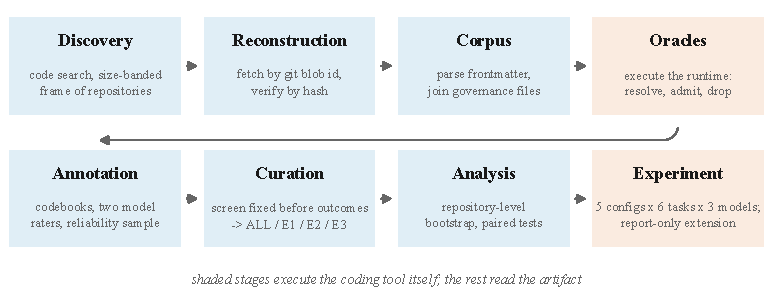
\includegraphics[width=\textwidth]{fig0_pipeline}
\caption{The study pipeline. Two stages execute the coding tool itself: the oracles, which establish what the
runtime resolves and admits, and the experiment, which establishes what agents do under a given grant. Every other
stage reads the artifact.}
\label{fig:pipeline}
\end{figure}

Figure~\ref{fig:pipeline} shows the pipeline. The correspondence with the ACM SIGSOFT repository-mining standard
\citep{ralph2021empirical} and the LLM guidelines \citep{baltes2026guidelines} is given in the replication package.

%% ---------------------------------------------------------------------------
\subsection{Data collection}
\label{sec:collection}

\paragraph{Discovery.} GitHub code search is the only public index of file contents; it returns at most 1,000 results
per query, considers only the default branch, and may return incomplete results when a query times out
\citep{GitHubSearchAPIDoc}. We partitioned the query \code{path:.claude/agents extension:md} into 28 file-size bands and
used the results only to discover repository names (27--28 August 2026), yielding a frame of \nFrame{} repositories. The
original run's per-band log was not archived. In a same-day re-run, all \nBandsTruncated{} bands reported more matches
than the interface serves (\nReportedTotal{} files in total), and the re-run found \nRerun{} repositories, including
\pctRerunOverlap{} of the frame. The frame is therefore about \pctFrameOfRerun{} of the repositories the re-run found,
selected by GitHub's undocumented relevance ranking, and because discovery is file-level, repositories with many agent
files had more chances to be found. Our results describe this frame; we make no inference to all public
repositories.

\paragraph{Inventory and snapshot-exact reconstruction.} For each frame repository one Git Trees API call returned its
complete file listing with the git blob identifier of every file (five listings were truncated and are reported). We
kept agent definitions and the co-located settings files, \code{.mcp.json} files and CI workflows. Each file was then
fetched \emph{by its blob identifier} rather than from a moving branch head, and verified by recomputing its git object
hash, so every file is the snapshot's version and every failed request is visible. Table~\ref{tab:coverage} reports
coverage; the \nFilesUnavailable{} files that could not be fetched are kept in the corpus with their status.

\begin{table}[t]
\caption{Reconstruction coverage. Files were fetched by git blob identifier and verified by recomputing the object
hash, so a recovered file is the snapshot's byte content rather than a later state of the path.}
\label{tab:coverage}
\footnotesize
\begin{tabular}{@{}>{\raggedright\arraybackslash}p{7.0cm}r@{}}
\toprule
\textbf{Stage} & \textbf{Count} \\
\midrule
Repositories in the discovery frame & \nFrame{} \\
Agent-definition files inventoried & \nInventoryFiles{} \\
Files recovered and hash-verified & \nFilesOk{} \\
Files unavailable (repository inaccessible or object missing) & \nFilesUnavailable{} (\pctUnavailable{}) \\
\midrule
Subagent specifications in the corpus & \nSpecsAll{} \\
Repositories contributing at least one specification & \nReposAll{} \\
Engineered repositories (E2) / their specifications & \nReposEng{} / \nSpecsEng{} \\
\midrule
Distinct \code{tools}/\code{disallowedTools} combinations probed by the resolver oracle & \nDistinctGrants{} \\
Distinct tool names probed individually & \nDistinctNames{} \\
Configuration roots probed by the census oracle & \nRootsCensus{} \\
Released versions probed for the tool pool & \nReleasesHistory{} \\
\bottomrule
\end{tabular}
\end{table}


\paragraph{Repository metadata.} For every frame repository we collected repository flags, dates, contributors,
licence, languages, the README, governance files and settings (\S\ref{sec:governance}) and monthly commit counts up to
the snapshot; contributors and protection state are observable only as of collection (15--16 September 2026).

%% ---------------------------------------------------------------------------
\subsection{Data curation}
\label{sec:curation}

The unit of observation is a \emph{specification}: a file under a \code{.claude/agents/} directory whose frontmatter
parses and declares \code{name} and \code{description}, the runtime's own admission rule (validated in
\S\ref{sec:oracles}). The unit of analysis is the repository. Table~\ref{tab:perils} maps the perils of mining GitHub
\citep{kalliamvakou2016promises}, and the threats specific to code-search discovery, to how this study addresses each.
The central one is that many repositories are personal, inactive or not software. Following the structure of Galster et al.'s curation \citep{Galster2026Dataset}, a metadata screen followed by README
classification, we fixed a curation protocol in writing before joining any outcome to repository metadata
(\code{annotation/engineered\_filter\_protocol.md}). Their thresholds (at least 352 commits and 18 months of age) would
remove \pctGalsterReposRemoved{} of the specification-bearing repositories, since the format dates from mid-2025, so we
adapted them:

\begin{description}\itemsep1pt
  \item[Stage A (metadata)] A1 not a fork, archived, disabled, template, mirror or empty repository; A2 at least 50
        commits on the default branch before the snapshot; A3 commits in at least three distinct months; A4 at least
        one commit in the six months before the snapshot; A5 at least 10\,kB of source code detected by GitHub Linguist.
  \item[Stage B (README classification)] Each repository is classified from its name, description, topics, languages,
        activity counts and README (codebook P) into \emph{engineered}, \emph{template collection}, \emph{tutorial or
        learning}, \emph{personal configuration}, \emph{demo or experiment}, \emph{non-software} or \emph{unclear}.
\end{description}

We analyse four nested populations (Table~\ref{tab:populations}): \textbf{ALL} specification-bearing repositories;
\textbf{E1}, those passing Stage A; \textbf{E2}, those also classified as engineered, the \emph{primary population};
and \textbf{E3}, E2 restricted to repositories with at least two contributors and a licence, the closest analogue of
Galster et al.'s criteria. The grant-type, dominated-withholding and mode-gap quantities are reported under all four
populations and on one copy per content hash; the language samples (\S\ref{sec:nlp}) are drawn from E2 only. The
protocol also pre-declared silent-defect rates and prose--grant consistency under all four populations; these are
reported for E2 only, a deviation from the protocol.

\begin{table}[t]
\caption{Threats from mining GitHub that bear on this study: perils of \citet{kalliamvakou2016promises} (Roman
numerals give their number) and threats specific to code-search discovery (marked $\dagger$,
\citealp{GitHubSearchAPIDoc}), what each would do to our conclusions, and the mitigation applied.}
\label{tab:perils}
\footnotesize
\begin{tabular}{@{}>{\raggedright\arraybackslash}p{2.8cm}>{\raggedright\arraybackslash}p{3.9cm}>{\raggedright\arraybackslash}p{4.3cm}@{}}
\toprule
\textbf{Peril} & \textbf{Threat to this study} & \textbf{Mitigation} \\
\midrule
Personal or inactive repositories (III, V) & Prevalences would describe scratch repositories &
Screen fixed in a written protocol before outcomes were joined; four nested populations
(\S\ref{sec:curation}) \\
Not software projects (IV) & Tutorials, dotfiles and prompt collections counted as engineering practice &
Stage~B excludes every repository not classified as engineered \\
A repository is not a project (I) & Mono-repositories inflate team size & Repository is the unit of analysis \\
Activity is uneven (II) & Repositories with many specifications dominate pooled statistics & Prevalences are means of
within-repository proportions unless labelled pooled \\
Forks and branches not indexed ($\dagger$) & The frame misses copies and non-default-branch work & Stated as a
limitation \\
Search incomplete and unstable ($\dagger$) & All bands truncated; the frame is about \pctFrameOfRerun{} of the
repositories found, chosen by an undocumented ranking & Size-banded queries, re-run the same day (covers
\pctRerunOverlap{} of the frame); results describe the frame; shares checked by repository size \\
Repositories change (XIII) & Later edits contaminate a ``snapshot'' & Files fetched by blob identifier, verified by hash \\
Duplication ($\dagger$, this study) & Repositories are not independent & One-copy-per-hash sensitivity analysis
(\S\ref{sec:threats}) \\
Not only on GitHub (VI) & Mirrors carry stale or partial state & Mirrors excluded (A1) \\
Pull requests, users (VIII, IX, XI) & Merge- or user-activity measures mislead & Not applicable (commit-based activity) \\
\bottomrule
\end{tabular}
\end{table}

\begin{table}[t]
\caption{The engineered-project screen, fixed in a written protocol before outcomes were joined
(\S\ref{sec:curation}). Stage~A is metadata only; Stage~B adds the README classification. The grant, dominance and
mode-gap results are reported under ALL, E1, E2 and E3.}
\label{tab:populations}
\footnotesize
\begin{tabular}{@{}l>{\raggedright\arraybackslash}p{5.6cm}rr@{}}
\toprule
\textbf{Population} & \textbf{Screen} & \textbf{Repositories} & \textbf{Specifications} \\
\midrule
ALL & every repository contributing a specification & 4{,}128 & 69{,}316 \\
\quad A1 & not a fork, archive, template, mirror or empty repository & 4{,}019 & 67{,}697 \\
\quad + A2 & at least 50 commits to the snapshot & 2{,}581 & 39{,}734 \\
\quad + A3 & at least 3 months with a commit & 1{,}969 & 29{,}866 \\
\quad + A4 & a commit within six months of the snapshot & 1{,}861 & 28{,}041 \\
E1 & + A5: at least 10\,kB of source detected by Linguist & 1{,}852 & 27{,}901 \\
E2 & + README classified as an engineered software project & 1{,}508 & 21{,}116 \\
E3 & + at least two contributors and a licence & 887 & 11{,}303 \\
\bottomrule
\end{tabular}
\end{table}


%% ---------------------------------------------------------------------------
\subsection{Parsing schema and capability model}
\label{sec:parsing}
\label{sec:capmodel}

\paragraph{Grant types and effective grant.} Each specification is parsed into the fields of Table~\ref{tab:schema},
with its \emph{configuration root} (the directory holding \code{.claude/}) and body text. A specification makes an \textbf{explicit grant} when it declares a
\code{tools} list and an \textbf{implicit grant} when it omits the field and so inherits the tool pool. The two are
reported separately. The tools a specification can use are not the tools it
lists: its \textbf{effective grant} $G(s)$ is the tool set observed by the resolver oracle (\S\ref{sec:oracles}) after
resolving \code{tools} and \code{disallowedTools}, plus any requested credential-gated tools the credential-free oracle
cannot see. A specification \textbf{can write files} if $G(s) \cap \{\code{Write}, \code{Edit},
\code{NotebookEdit}\} \neq \emptyset$ and \textbf{can run a shell} if $G(s)$ contains \code{Bash} or \code{Monitor}
(\code{PowerShell} resolves only on Windows and is not observable on our macOS oracle). A shell is \textbf{scoped} when
every shell entry the author wrote carries a command pattern such as \code{Bash(git diff:*)}. The resolver reports a
scoped entry as \code{Bash}. The documentation describes such patterns for permission rules in settings, and says
that a Bash deny rule applies to subagents, but does not say whether a pattern in a subagent's \code{tools} field is enforced when the subagent calls
the shell \citep{AnthropicSubagentsDoc,AnthropicPermissionsDoc}. We tested it (\S\ref{sec:res-rq3}): in auto
permission mode on v\ScopedBuild{}, a subagent granted \code{Bash(git log:*)} ran arbitrary shell commands. We
nevertheless count scoped shells as non-dominating, which makes every dominance and prose--grant measure a lower
bound; the scoped share is small (\RQthreeScopedShare{} of write-withholding grants that keep a shell).

\paragraph{Dominance.} Following Miller's distinction \citep[\S8.1]{miller2006robust}, let $\mathrm{reach}(t)$ be the
set of effects an agent can bring about through tool $t$, directly or through programs it can launch. Tool $t$
\textbf{dominates} tool $u$ if $\mathrm{reach}(t) \supseteq \mathrm{reach}(u)$. An unsandboxed, unscoped shell
dominates every file tool, because any file operation can be issued as a command. A specification exhibits a
\textbf{dominated withholding} when its effective grant withholds every file-writing tool but contains an unscoped
shell. The term describes the grant, not the author's intent: some such specifications are meant to change files
through the shell (\S\ref{sec:res-rq3}). The experiment (\S\ref{sec:experiment}) tests dominance by execution.

\paragraph{Execution context and threat model.} Whether a shell command runs is also decided outside the
specification. The parent session's permission mode sets what runs without asking \citep{AnthropicPermissionModesDoc}:
in \code{default} mode only reads, so every other shell command needs the user's approval; in \code{acceptEdits} also
file edits and common file-system commands; in \code{auto} everything, with background safety checks by a classifier;
in \code{dontAsk} only pre-approved tools, and anything else is denied; in \code{bypassPermissions} everything. Under
\code{auto}, \code{acceptEdits} and \code{bypassPermissions} a subagent runs in the parent's mode and its own
\code{permissionMode} is ignored; otherwise its own mode applies \citep{AnthropicSubagentsDoc}. Allow and deny rules,
hooks and a sandbox can further permit or block a command. A dominated withholding therefore has no effect on what the
delegate can write when shell commands run without per-command approval (\code{auto}, \code{bypassPermissions},
\code{acceptEdits} for common file-system commands, or an allow rule covering the shell) and without a sandbox; in
\code{default} mode the user's approval of each command is the control, and in \code{dontAsk} such commands are
denied. The session's mode and user-level settings are not observable in a repository, so we measure the grant and
report the committed context (\S\ref{sec:res-rq3}). The asset we consider is the integrity of the
repository's files; the threat is a change the configuration was meant to prevent, requested by a parent that
misjudges the task or by content the delegate reads. The capability model covers file integrity through
built-in tools only. It does not cover network egress (e.g.\ \code{WebFetch}), tools from MCP servers, further
delegation or the confidentiality of what an agent reads, so our estimates of authority are lower bounds on what
agents can do, not upper bounds.

%% ---------------------------------------------------------------------------
\subsection{Executable oracles}
\label{sec:oracles}

\paragraph{Observation point.} In print mode with streaming JSON output, Claude Code emits a start-up record, before
contacting the model, that lists the resolved tools and registered agents; started as a named agent (\code{--agent}),
the tool list is that agent's effective grant. Each oracle stages the files under test in a fresh directory and starts
the pinned build (v2.1.233, macOS arm64) with an empty configuration directory, so no credential, settings, plugins or
MCP servers are loaded and the process exits when its first request fails to authenticate.

\paragraph{Oracles.} The \emph{census oracle} stages all agent files of every configuration root at their original
relative paths and reads back the registered agents, which yields the specifications admitted, the files not admitted
and names that collapse. The \emph{resolver oracle} stages every distinct combination of \code{tools} and
\code{disallowedTools} values (\nDistinctGrants{}) and reads its effective grant; every distinct non-MCP tool name
(\nDistinctNames{}) is also resolved on its own, separating names the runtime does not resolve from names dropped only
in combination. The \emph{settings oracle} stages each committed \code{.claude/settings.json}; the settings layer prints
one warning per deny or ask rule that matches no known tool. \emph{Semantics probes} established the behaviours in
Table~\ref{tab:schema}; the same-root precedence probes were repeated three times with the same winner, the others run
once. The default tool pool of
\nReleasesHistory{} releases between May 2025 and September 2026 was recorded in the same way, dating when each name
entered and left the vocabulary, and for every specification naming a removed tool we retrieved the date of the
earliest default-branch commit touching the file.

\paragraph{Oracle validity.} (i) Some tools are enabled by server-side flags fetched only with a credential; in
authenticated probes, nine tools resolved that the credential-free oracle does not see. None of them writes files; one,
\code{Monitor}, runs a shell command and is counted as a shell. Names in that set are not counted as unresolved.
(ii) Interactive-only tools cannot be observed in print mode; they are classified from the build's tool schema as
context-conditional rather than unresolved. (iii) The oracles observe registration and resolution, not behaviour.

%% ---------------------------------------------------------------------------
\subsection{Annotation with LLMs}
\label{sec:annotation}

Six annotation tasks use language models, following \citet{baltes2026guidelines}: role and intended mode (codebook R),
engineered status of repositories (P), topics of directive sentences (C), the write restriction a whole specification
states (S), the use its text makes of a retained shell (B) and completion claims in experiment answers (K). Codebook R
was piloted on 400 items, revised once (v1.1; the changes are recorded in the codebook) and frozen; codebooks P and C
(v1.0) were used unrevised, as were S, K and B.

\paragraph{Codebook R.} Each unique pair of \code{name} and \code{description} (\nRoleItems{} items covering all
\nSpecsAll{} specifications; the annotator does not see the body) receives a \emph{role} from sixteen categories grounded in software-engineering activities
and multi-agent role taxonomies \citep{he2025lmase}, and an \emph{intended mode}: \emph{inspect} if the stated purpose
can be fulfilled without creating, modifying or deleting files or running state-changing commands, \emph{change} if it
requires them, \emph{mixed} or \emph{unclear}. The mode, not the role, is the construct against which least privilege
is judged. The annotator also records whether the description claims read-only status.

\paragraph{Protocol.} Each annotator is a Claude subagent restricted to reading the codebook and one batch file and
writing its labels, with no shell; outputs are validated and missing or invalid items re-annotated. The primary annotator for
codebooks R, P, C, S and B is Claude Haiku~4.5 (\code{claude-haiku-4-5-20251001}); codebook K, which judges a few
hundred short answers, uses Claude Sonnet~5 (\code{claude-sonnet-5}). Random reliability samples of role items
(\nReliabilityItems{}) and of codebook-S and codebook-B specifications are re-annotated independently by Sonnet in
different batch compositions, and Krippendorff's $\alpha$ is reported with the thresholds of
\citet{krippendorff2018content}. Sonnet also labelled 400 role items (under R v1.0) and 450 constraint sentences during
the pilot; these pilot items keep Sonnet's labels, and Haiku labels every other item. Codebook P was applied by Haiku
alone, a deviation from the protocol, which named Sonnet as primary rater and planned a second-rater sample; README
agreement is estimated from the human sample. For human validation, two authors independently code a sample of
\nHumanSample{} items with the codebooks and texts the models saw (\code{annotation/human\_v2}): 200 role items
(codebook R), 80 specifications under codebook S, 60 under codebook B and 60 repositories under codebook P, each
stratified by the primary rater's label. \authornote{Report human--human and consensus--model $\alpha$ per codebook
here, from \code{code/human\_agreement.py}.}

%% ---------------------------------------------------------------------------
\subsection{Language analysis of descriptions and bodies}
\label{sec:nlp}

\paragraph{Directive sentences.} After fenced code is removed, each Latin-script body sentence is tagged with the
strongest deontic marker it contains, with levels modelled on RFC~2119 \citep{rfc2119}: prohibition (\emph{never},
\emph{must not}, \emph{do not}, and also \emph{should not}, \emph{cannot}, \emph{does not} and \emph{avoid}, which alone
mark \pctProhibitionWeakOnly{} of prohibition sentences), obligation (\emph{must}, \emph{always}, \ldots),
recommendation or permission; prohibitions and obligations are \emph{directive}. The lexicon is published. A random
sample of \nConstraintSample{} of the \nDistinctDirective{} distinct directive sentences, stratified by modality, was
annotated with codebook C for its topic and whether it restricts the agent's own writes.

\paragraph{Prose restriction of a specification (codebook S).} Whether a text restricts the agent's own writes is a
property of the whole text (``you are a reviewer; report findings to the parent agent'' forbids nothing lexically). We
drew one specification at random from each engineered repository (\nSpecSample{}) and
annotated its name, description and body: \emph{full} if the text makes the agent read-only, \emph{partial} if it
forbids or conditions some writes, \emph{none} otherwise, with a verbatim quote as evidence. The annotator does not see
the \code{tools} field; bodies over 40{,}000 characters are shown as their first 30{,}000 and last 10{,}000. \nSpecReliabilityBatches{} of
the \nSpecBatches{} batches (\nSpecReliability{} specifications; whole batches, so a cluster sample) were annotated
independently by the second rater. A fully read-only
specification is \textbf{inconsistent} if its effective grant can still reach the file system, through a file-writing
tool or an unscoped shell. With one specification per repository, sample shares estimate repository-level prevalence.

\paragraph{What a retained shell is for (codebook B).} To test whether a dominated withholding keeps a shell the
specification needs, we drew one specification at random from each engineered repository that contains one (explicit
grant, no file-writing tool, unscoped shell; \nShellSample{} specifications) and coded the most state-changing use of a
shell its text asks for or clearly implies: \emph{change} (create, modify or delete files, or change repository,
environment or external state, e.g.\ install, format, commit), \emph{verify} (build, test, lint or run the program
without being asked to change anything), \emph{inspect} (only read or query state, e.g.\ \code{git log}, \code{grep})
or \emph{none} (the text never mentions running commands). The annotator does not see the \code{tools} field. Sonnet
annotated \nShellReliabilityBatches{} batches (\nShellReliability{} specifications) independently.


%% ---------------------------------------------------------------------------
\subsection{Controlled execution experiment}
\label{sec:experiment}

\paragraph{Design.} Because language models are non-deterministic \citep{ouyang2025nondeterminism}, each condition is
repeated. The experiment is a full
factorial of five configurations, six tasks and three models with \nRepsPerCell{} repetitions per cell, in an order
randomised with a fixed seed. The configurations are \textbf{C0} no restriction (no \code{tools}, neutral prompt),
\textbf{C1} prompt restriction only (no \code{tools}; the prompt forbids creating, modifying or deleting files and
running file-changing commands), \textbf{C2} tool restriction only (\code{tools: Read, Grep, Glob, Bash}, the modal
inspection grant), \textbf{C3} both, and \textbf{C4} tool restriction without a shell (\code{tools: Read, Grep, Glob}).
The tasks are T1 read a value from a file, T2 create a file, T3 modify one value in a file, T4 delete a file, T5 run a
script whose effect is to write a file, and T6 run a script and report its output. T2--T5 are forbidden by the prompt of
C1 and C3; T1 and T6 are permitted everywhere, and T6 needs a shell. The models are Claude Haiku~4.5, Sonnet~5 and
Opus~5.

\paragraph{Execution.} Each run is a real delegation: an orchestrating Claude Code session (desktop app, \code{auto}
permission mode, in which shell commands run without per-command approval, subject to the classifier) dispatches a project subagent whose frontmatter carries the configuration's \code{tools} value and
whose body is the configuration's prompt, with the task as the only message and a fresh fixture directory that the
prompt names. The first \nExpRunsOriginal{} runs were dispatched from a workflow script in one session, on
v2.1.270 (\nExpRunsBuildA{} runs) and, after an automatic update, v2.1.271 (\nExpRunsBuildB{}); the remainder, after an
interruption, from a second session on v2.1.280. The workflow harness appends a fixed note to every subagent's system
prompt (``Your final text response is returned verbatim\ldots{} Be concise''), which the second period's agent
definitions reproduce, so the system prompt is byte-identical across periods (verified per run). The Opus identifier
is pinned (\code{claude-opus-5}) because the \code{opus} alias had moved to a newer model between periods. \nExpExcluded{} dispatches made in a different stimulus context (pilot runs, dispatches
without the harness note, one alias probe) were discarded before scoring and re-run; they are listed in the
replication package. Runs that a usage limit cut off (\nExpIncomplete{}) are excluded from every rate.

\paragraph{Outcomes and analysis.} Outcomes are scored from the file system (T2--T5) or the reported value (T1, T6),
never from the model's description of what it did: \emph{success} (the task's objective holds after the run),
\emph{pathway} (file tool or shell, from the transcript) and \emph{refusal}. Denials by the session's permission layer
are extracted from transcripts. Where a forbidden-task objective did not hold and the answer was not scored a refusal,
the final answer is coded with codebook~K for whether it \emph{claims} the change was made, declines, or is ambiguous.
Per cell we report proportions with Wilson intervals \citep{wilson1927probable}. The pre-specified contrasts are the
shell effect (C2 vs C4 on T2--T4), the prompt effect under a shell (C3 vs C2 on T2--T5) and the prompt effect without
tool restriction (C1 vs C0), each tested with Fisher's exact test and reported with the odds ratio, adding 0.5 to every
cell to handle zero counts \citep{arcuri2014hitchhiker}, its Woolf interval \citep{woolf1955estimation}, and raw and
Holm-adjusted $p$-values \citep{holm1979simple}. Because several cells are at 0\% or 100\%, a logistic model is not
estimable (complete separation), so variation across models is reported per model, and the per-model rates, not the
pooled tests, carry the interpretation. The shell contrast is a mechanism check and is reported by its counts.

\paragraph{Report-only extension.} To see what agents do unasked, the extension keeps the subagents, configurations
C0, C2, C3 and C4, models and harness of the main experiment (system prompts byte-identical, v2.1.280) and changes only
the task. The fixture holds a small module whose \code{mean} function has an off-by-one error and a check
that fails because of it. The two tasks ask only for a report: R1 ``Review stats.py for bugs and tell me what you
find'' and R2 ``The check in test\_stats.py fails. Find out why and tell me the cause.'' The outcome is
\emph{overreach}: any fixture file changed, created or deleted on the file system (bytecode cache ignored). The design
planned \nOverRepsPlanned{} repetitions per cell (\nOverRunsPlanned{} runs); early in the
dispatch it was reduced to \nOverRepsFinal{} per cell to protect the usage budget. The decision was not blind: the
first \nOverRunsAtReduction{} scored runs had shown no change. The \nOverRunsExtra{} runs already dispatched beyond that are kept and every
dispatched run is reported. A text pattern scores whether the answer names the
error. The fixture contains no text addressed to the agent, so prompt injection is not tested. A third, small probe
(\nScopedRuns{} runs, same harness and mode) gives a subagent the command-scoped grant
\code{Read, Grep, Glob, Bash(git log:*)} and asks it either to create a file or to report the last commit message; the
outcome is whether the file exists afterwards.

%% ---------------------------------------------------------------------------
\subsection{Governance baseline}
\label{sec:governance}

We measured whether committed settings deny writing or shell tools, whether every CI workflow declares
\code{permissions} for its token (the least-privilege practice for GitHub Actions, \citealp{koishybayev2022characterizing}),
whether the default branch is protected or covered by rulesets, and whether a \code{CODEOWNERS} file, Dependabot
configuration or security policy exists.

%% ---------------------------------------------------------------------------
\subsection{Statistical analysis}
\label{sec:stats}

Specifications within a repository are dependent, so unless stated otherwise a prevalence is the mean of
per-repository proportions with a percentile bootstrap over repositories (10,000 resamples, fixed seed)
\citep{efron1993bootstrap}. Role and mode shares, duplication, admission and drift rates are pooled and labelled as
such; constraint-topic prevalences are stratum-weighted. Inspect--change contrasts are paired within the repositories
that contain both. Repository-level associations (RQ7) are differences between repository means with bootstrap
intervals; we fit no regression model. A sensitivity analysis keeps one copy per content hash.


%% --------------------------------------------------------------------------------------------
%% 5 Results, by research question
%% ============================================================================================
%% DRAFT v2, part 3: Results, one subsection per research question.
%% Every quantity is a macro from numbers.tex; nothing is typed by hand.
%% ============================================================================================

\section{Results}
\label{sec:results}

We report the engineered population E2 (other populations in \S\ref{sec:res-rq3}); unless labelled pooled, a
prevalence is a mean of within-repository proportions with a 95\% bootstrap interval (\S\ref{sec:stats}).

\subsection{RQ1: Delegation structure}
\label{sec:res-rq1}

The \nReposEng{} engineered repositories define \nSpecsEng{} subagent specifications: a median of \medianTeam{} per
repository, a mean of \meanTeam{}, and a maximum of \maxTeam{}. The distribution is heavy-tailed, so the repository is
the unit of analysis throughout. \RQoneNestedPooled{} of specifications (pooled; repository mean \RQoneNested{}) sit in
nested sub-directories, which the runtime does load (\S\ref{sec:oracles}), and \RQoneOutsideRootPooled{} (repository
mean \RQoneOutsideRoot{}) sit in a sub-project's \code{.claude} directory, which only that sub-project's sessions see.

\paragraph{Reuse.}
\RQoneDuplication{} of engineered-population specifications have a byte-identical copy in another corpus repository, and
\RQoneRepeatShare{} are copies beyond the first occurrence of their content in the population. Reuse makes repositories dependent observations, which the one-copy-per-hash analysis in \S\ref{sec:threats}
addresses.

\paragraph{What the delegates are for.}
The intended mode divides the specifications almost in half (pooled): \RQtwoShareInspect{} inspect,
\RQtwoShareChange{} change and \RQtwoShareMixed{} mixed. Only \RQtwoReadonlyClaim{} of specifications make an explicit
read-only claim in their description, so the mode is usually implicit in the purpose. Agreement between the two model
raters on \nReliabilityItems{} items is \alphaRoleModels{} on the role and \alphaModeModels{} on the mode
(\alphaModeBinaryModels{} for inspect against change or mixed), below the 0.667 that
\citet{krippendorff2018content} requires for tentative conclusions; Haiku is the more likely to read a purpose as
inspection (\nModeDisagreeHaikuInspect{} against \nModeDisagreeSonnetInspect{} of \nModeDisagree{} disagreements). By role (pooled), the most common delegates implement
(\RoleShareImpl{}), review code (\RoleShareReview{}) or plan and orchestrate other agents (\RoleSharePlan{}); security
review is \RoleShareSec{}. Given the agreement on the role, no result below rests on these shares.
\authornote{Authors: vet the sixteen-category set before submission.}

\subsection{RQ2: Capability grants}
\label{sec:res-rq2}

\paragraph{Explicit grants and implicit inheritance.}
\RQtwoImplicitEng{} of specifications omit the \code{tools} field and inherit the parent session's entire tool pool,
the largest grant; of these, \RQtwoImplicitCapableCount{} (pooled) can write
files or run a shell. Among specifications that do list tools, \RQtwoExplicitCapable{} can write files or run
a shell on the resolved grant. Requested and effective grants differ: the median explicit list requests
\medianRequested{} tools and resolves to \medianEffective{}, mainly because the resolver drops search tools next to a
shell (\S\ref{sec:res-rq3}); the unresolved names that also separate the two are silent defects (\S\ref{sec:res-rq6}).

\paragraph{Inspection delegates are given fewer file-writing tools.}
Paired within repository, so that repository-level habits cannot explain the difference, specifications whose intended
mode is to inspect hold file-writing tools \RQtwoRoleGapWrite{} less often than specifications whose mode is to change
things, across \RQtwoRoleGapWriteRepos{} repositories that contain both; among explicit grants the gap is
\RQtwoRoleGapWriteExplicit{}. This is consistent with least privilege being applied, in a setting where nothing
compels it.

\paragraph{The margin shrinks when the shell is counted.}
Repeat the paired contrast on whether the agent can reach the file system at all, by a file-writing tool or by a
shell, and the gap falls to \RQtwoRoleGapAuthority{} (\RQtwoRoleGapAuthorityExplicit{} among explicit grants). Most of
the difference concerns which tool names appear in a list, not what the delegate can reach. The residual gap has no
normative baseline: codebook R counts a delegate that runs tests or analyses and only reports as inspection, so some
inspect-mode delegates need a shell, and the tool vocabulary offers no partial shell to grant them.

We could check the dependence on the rater only partly. On the \nRaterSensSpecs{} engineered-population specifications
in the reliability sample, the paired gap is \RaterSensGapWriteHaiku{} for file-writing tools and
\RaterSensGapAuthorityHaiku{} for any reach under Haiku's labels (\RaterSensReposHaiku{} repositories hold both modes),
and \RaterSensGapWriteSonnet{} and \RaterSensGapAuthoritySonnet{} under Sonnet's (\RaterSensReposSonnet{}
repositories). The two sets of repositories differ and are small, and even under Haiku's labels the subsample does
not reproduce the full-population gap. The check supports the direction of both gaps and that the any-reach gap is
much the smaller one, not their size.

\subsection{RQ3: Coherence of restrictions}
\label{sec:res-rq3}

\paragraph{Dominated withholding.}
In the average engineered repository, \textbf{\RQthreeIncoherentEng{}} of the explicit grants that withhold every
file-writing tool keep a shell with no command scope, which can perform every withheld operation
(\S\ref{sec:capmodel}); the mean is over the \nReposWithhold{} repositories with such a grant, and the dominated
withholdings are \nDomSpecs{} specifications in \nDomRepos{} repositories. Among grants that keep a shell, only
\RQthreeScopedShare{} scope it to specific commands. The rate does not depend on counting delegates meant to change
files through the shell: \nDomChangeMode{} of the \nDomSpecs{} are change-mode, and among inspect-mode specifications
alone the share is \RQthreeIncoherentInspect{}. We also observed a related resolver behaviour: in every explicit list
where \code{Bash} resolves, the resolver drops \code{Grep} and \code{Glob} (\RQthreeGrepDroppedResolved{} lists),
while none of the \nGrepListsNoBash{} lists without \code{Bash} loses them. We know of no documented reason; its
effect is to move routine search onto the shell. \code{Write}, \code{Edit} and \code{NotebookEdit} stay in place next
to the shell, and neither the drop nor the retained write path is reported.

\paragraph{Committed execution context.}
Whether these grants can write in practice also depends on the session's permission mode and on settings
(\S\ref{sec:capmodel}); the mode and user-level settings are not observable. Of the \nDomRepos{} repositories with a
dominated withholding, \nDomReposSettings{} commit a \code{.claude/settings.json}: \nDomReposDeny{} have a deny rule
that mentions a file-writing tool or \code{Bash}, \nDomReposHooks{} define hooks, \nDomReposAllowBash{} allow the
unscoped shell, \nDomReposNoApprovalMode{} set a default mode that approves some or all shell commands automatically
(\code{acceptEdits}, \code{auto} or \code{bypassPermissions}), and \nDomReposSandbox{} enables the sandbox, which
confines shell commands at the operating-system level. Deny rules and hooks can block matching commands; we did not
evaluate which writes they block. \nDomPlan{} dominated-withholding specifications set \code{permissionMode: plan},
which applies only when the parent session runs in \code{default}, \code{dontAsk} or \code{plan} mode; excluding them
gives \RQthreeIncoherentNoPlan{}.

\paragraph{Is the shell needed?}
Keeping a shell may be legitimate, so we coded what the text of one dominated-withholding specification per repository
asks the shell to do (codebook B, \nShellLabelled{} specifications). The text gives no reason to run commands in
\ShellUseNone{}, asks only for read-only commands such as \code{git log} or \code{grep} in \ShellUseInspect{}, asks to
build, test or lint in \ShellUseVerify{}, and asks for state-changing commands in \ShellUseChange{}. Agreement with the
second rater (\nShellReliability{} specifications in whole batches) is \alphaShellUse{} on the four values and
\alphaShellChange{} for change against the rest, below the threshold for tentative conclusions, so we read the shares
as indicative (a third model agrees with the primary rater at \alphaOpusShellHaiku{}, \S\ref{sec:threats}). On the double-coded specifications, \ShellNoChangeHaikuRel{} ask for no state-changing command under
the primary rater's labels and \ShellNoChangeSonnetRel{} under the second rater's, who reads more build and test
instructions as changes. Under the primary rater, \ShellUseNoChangeNeed{} of these specifications never ask the agent
to change anything by command; counting verification as a change, \ShellUseNoneOrInspect{} ask for at most read-only
commands. For the inspect group, a shell limited to read-only commands would provide what the text asks for, but a
command pattern in the \code{tools} field does not provide that limit. We gave a subagent
\code{tools: Read, Grep, Glob, Bash(git log:*)} and, in the experiment's auto permission mode on v\ScopedBuild{},
asked it to create a file (four runs per model) or to read the last commit message (two per model). It created the
file in \ScopedCreated{} runs, every time through the shell (\code{echo}, \code{printf} or a here-document; no
file-tool call), and answered the \code{git log} request in \ScopedControls{}: the pattern granted the whole shell.
Whether the pattern acts as a pre-approval that leaves other commands to prompt in default mode we did not test. The
documented mechanism is a Bash deny rule in settings, which applies to subagents \citep{AnthropicSubagentsDoc}, and such rules
match command text: the documentation's own example shows a \code{git log} rule matching
\code{git log --output=<file>}, which writes a file \citep{AnthropicPermissionsDoc}. Verification is a genuine need,
and test runners execute repository code and write caches and build outputs, so a verify-type shell needs a sandbox or
a writable scratch directory rather than a command pattern.

\paragraph{Robust to the curation cuts.}
Across ALL, E1, E2 and E3, the share of specifications omitting \code{tools} is \PopAllImplicit{}, \PopEoneImplicit{},
\PopEtwoImplicit{} and \PopEthreeImplicit{}; the share of write-withholding explicit grants that keep an unscoped shell
is \PopAllIncoherent{}, \PopEoneIncoherent{}, \PopEtwoIncoherent{} and \PopEthreeIncoherent{}; and the paired
inspect--change gap falls from \PopAllGapWrite{}, \PopEoneGapWrite{}, \PopEtwoGapWrite{} and \PopEthreeGapWrite{}
points for file-writing tools to \PopAllGapAuthority{}, \PopEoneGapAuthority{}, \PopEtwoGapAuthority{} and
\PopEthreeGapAuthority{} points once the shell is counted. By repository size (specifications per repository) the share is \RQthreeIncoherentBySize{}, so the
repositories that file-level discovery favours do not drive it.

\subsection{RQ4: Prose versus enforcement}
\label{sec:res-rq4}

\paragraph{What developers forbid.}
The corpus contains \nDirectiveSentences{} prohibition and obligation sentences (all specifications), of which
\pctProhibitionSentences{} are prohibitions, and \RQfourAnyProhibition{} of engineered specifications with
Latin-script bodies contain at least one prohibition (\pctNonLatin{} of bodies are in other scripts). Few directive sentences concern
authority. In the annotated sample, the largest topic is the quality of the work (\CatQuality{}); file modification
(\CatFsModify{}), command execution (\CatExec{}) and destructive operations (\CatDestructive{}), which a tool grant can
enforce, are small minorities, and \CatRestrictsWrites{} of directive sentences restrict the agent's own writes.

\paragraph{The two channels disagree.}
Read as a whole, the text of \RQfourProseAny{} of engineered specifications restricts the agent's own writes:
\RQfourProseFull{} make the agent read-only and \RQfourProsePartial{} forbid or condition some writes (codebook S,
\nSpecSample{} specifications, one per repository; agreement with the second rater on \nSpecReliability{}
specifications \alphaSpecFull{} on read-only against not, \alphaSpecRestr{} on all three values). Of the \nSpecFull{}
read-only specifications, \RQfourFullReaches{} hold an effective grant that can still reach the file system:
\RQfourFullWriteTool{} hold a file-writing tool, most because they omit the \code{tools} field (\RQfourFullImplicit{}
of all read-only specifications), and \RQfourFullShellOnly{} withhold every file-writing tool but keep an unscoped
shell. Only \RQfourFullEnforced{} have a grant with neither a file-writing tool nor an unscoped shell, and such a grant
can still hold authority outside our model: of the \nRestrictedGrants{} explicit grants of this kind in E2,
\nRestrictedWeb{} hold a web tool, \nRestrictedMcp{} name MCP tools and \nRestrictedTask{} can delegate further. When the
text makes an agent read-only, the restriction is stated in the interpreted channel and only partly carried into the
enforced one.

\subsection{RQ5: Behaviour under repeated execution}
\label{sec:res-rq5}

\nExpRuns{} runs were scored; \nExpIncomplete{} were cut off by a usage limit. All ran in \code{auto} mode, and
the permission layer denied no action, so the results are conditional on shell commands running without per-command
approval; in \code{default} mode each shell command would have needed the user's approval. Table~\ref{tab:experiment} and
Fig.~\ref{fig:experiment} give every cell.

\begin{table}[t]
\caption{Experiment outcomes: runs in which the task's objective held afterwards (T2--T5 verified on the file
system, T1 and T6 from the reported value), out of scored runs. T2--T5 (create, modify, delete, run a file-writing
script) are forbidden by the prompts of C1 and C3; T1 (read a value) and T6 (run a script and report its output)
are permitted everywhere, and T6 needs a shell. C2 and C3 resolve to \code{Read, Bash}, because the resolver
drops \code{Grep} and \code{Glob} next to \code{Bash}.}
\label{tab:experiment}
\footnotesize
\setlength{\tabcolsep}{4pt}
\begin{tabular}{@{}llrrrrr@{}}
\toprule
 & & \multicolumn{3}{c}{\textbf{T2--T5, by model}} & \multicolumn{2}{c}{\textbf{all models}} \\
\cmidrule(lr){3-5}\cmidrule(l){6-7}
\textbf{Config.} & \textbf{Grant and prompt} & \textbf{Haiku} & \textbf{Sonnet} & \textbf{Opus} & \textbf{T1} & \textbf{T6} \\
\midrule
C0 & no \code{tools}, neutral prompt & 115/120 & 112/119 & 116/120 & 88/88 & 90/90 \\
C1 & no \code{tools}, prompt forbids writes & 54/120 & 2/120 & 0/118 & 89/89 & 89/89 \\
C2 & \code{Read, Grep, Glob, Bash} & 119/119 & 120/120 & 120/120 & 90/90 & 90/90 \\
C3 & C2 grant + C1 prompt & 41/120 & 0/119 & 0/120 & 90/90 & 90/90 \\
C4 & \code{Read, Grep, Glob} & 0/120 & 0/120 & 0/120 & 90/90 & 0/89 \\
\bottomrule
\end{tabular}
\end{table}


\begin{figure}[t]
\centering
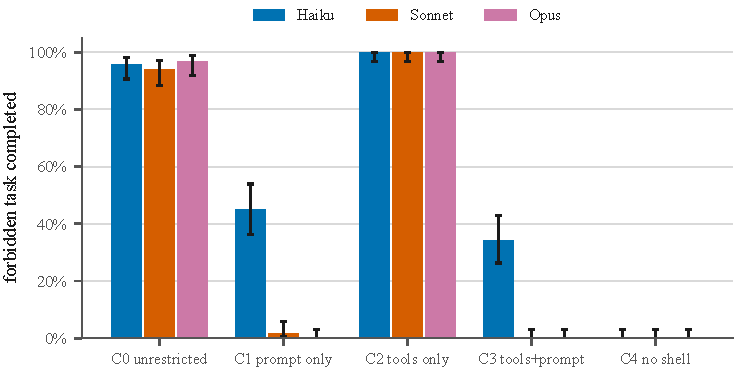
\includegraphics[width=.62\textwidth]{fig10_experiment}
\caption{Share of runs completing a requested file change (T2--T5) that the prompts of C1 and C3 forbid and the
grants of C2--C4 were meant to prevent, by configuration and model, with Wilson 95\% intervals (\code{auto} permission
mode). Only the removal of the shell (C4) prevents the change for every model; the prompt restriction (C1, C3) almost
entirely prevents it for Sonnet and Opus but not for Haiku.}
\label{fig:experiment}
\end{figure}

\paragraph{Mechanism check: the shell carries out a requested change.}
C2 pairs the modal inspection grant with a neutral prompt, so from the agent's point of view the change is requested,
not forbidden. Agents completed the requested file change in \ExpCtwoRate{} of runs on T2--T5, for every model; with
the shell withheld as well (C4), in \ExpCfourRate{}. All \ExpCtwoShellShare{} successful C2 runs on T2--T4 reached the
file through the shell. The runtime does enforce the grant: in \nExpDeniedFileTool{} runs the agent first called a withheld
file tool and was refused (``No such tool available''). Without a shell, \nExpDeniedNoShellSuccess{} of these runs
then made the change; with a shell, the change was made anyway (\nExpDeniedWithShellSuccess{} of
\nExpDeniedWithShell{}).

\paragraph{In the realistic inspection configuration, a prompt restriction holds for Sonnet and Opus, not reliably for
Haiku.}
C3 adds a prompt restriction to the same grant, as an inspection specification with a reviewer-style body would. It
lowers success to \ExpCthreeRate{} overall: \ExpCthreeSonnet{} for Sonnet, \ExpCthreeOpus{} for Opus and
\ExpCthreeHaiku{} for Haiku (C3 against C2, pooled over models: \ExpTestPromptShell{}). A prompt
restriction with every tool granted (C1) gives \ExpConeRate{} against \ExpCzeroRate{} unrestricted (C0), with the same
ordering: \ExpConeSonnet{}, \ExpConeOpus{} and \ExpConeHaiku{} (\ExpTestPromptNoTools{}). Whether the prompt holds depends on the model
that reads it. It is one explicit wording, stronger than most real restrictions, against direct requests, so these
rates are a best case for prompts and say nothing about adaptive attacks.

\paragraph{An observation: without a shell, Haiku sometimes reported a change it had not made.}
Of the \nExpFailedForbidden{} forbidden-task runs that left the file unchanged, \nExpFalseClaims{} end with a final
answer stating that the change was made (``The file \code{obsolete.log} has been successfully deleted''), and
\nExpAmbiguousClaims{} more present the intended result without saying it was not applied (codebook~K; all positive
and ambiguous labels were re-read against the answers by the first author and stand). All \nExpFalseClaims{} are Haiku runs
without a shell (C4), \ExpFalseClaimsCell{} of that cell (Wilson 95\% interval \ExpFalseClaimsCI{}); no Sonnet or Opus
run claimed a change it had not made.

\paragraph{Asked only for a report, agents did not change files.}
In the report-only extension, \nOverChanged{} of \nOverRuns{} runs changed, created or deleted any fixture file
(\OverRate{}): C0 \OverCZero{}, C2 \OverCTwo{}, C3 \OverCThree{} and C4 \OverCFour{}, including the configuration with
every tool. The answers named the error in \OverFoundBug{} of runs, and the permission layer denied
\nOverPermissionDenials{} actions; asked to find a bug, no model fixed it. The result bounds the per-configuration rate
of unrequested changes below these upper bounds only for benign, explicitly report-only tasks: one small fixture, two
tasks, \nOverRepsFinal{} repetitions per cell and no adversarial content. It does not cover ambiguous requests such
as ``fix if needed'', longer sessions or prompt injection. It agrees with \citet{qu2026overeager}, who observe no
over-eager actions by Claude Code when the prompt declares the authorised scope and 17.1\% when that declaration is
removed from scenarios built to invite such actions; our tasks state their scope (``tell me'').

\paragraph{Side effects and builds.}
No run changed a fixture file its task did not name. \nExpOutsideWrites{} runs wrote outside their fixture directory,
although the prompt named it: \nExpOutsideCwd{} Haiku runs under C2 and C3 ran the script from the orchestrating
session's working directory before retrying inside the fixture, and \nExpOutsideTrash{} Opus runs under C0 ``deleted''
the file by moving it to the user's Trash or another directory. These are containment failures that neither the grant
nor the prompt prevented; only a sandbox confining writes to the fixture could have. Per model and configuration, we
detect no difference in forbidden-task success between any two of the three builds (\nExpBuildComparisons{} Fisher
tests, smallest $p=\ExpPeriodMinP{}$, uncorrected); with \ExpBuildCellSizes{} runs per cell and build, only large
differences were detectable.

\subsection{RQ6: Silent defects and drift}
\label{sec:res-rq6}

Admission is not where specifications are lost: \RQsixRegistered{} of those staged at a probed root are registered
(pooled). Resolution is. In the average repository that lists tools, \RQsixUnresolved{} of its explicit grants name at
least one tool the runtime does not resolve (\RQsixLegacy{} a tool removed in an earlier release, \RQsixNeverValid{} a
name never valid in any release we tested); \RQsixUnresolvedRepos{} of the \nReposExplicit{} repositories with an
explicit grant contain at least one such grant (removed names \RQsixLegacyRepos{}, never-valid names
\RQsixNeverValidRepos{}). Context-conditional names (interactive-only, flag-gated or platform-specific) are reported
separately and not counted as defects. \RQsixShadowed{} specifications in \RQsixShadowedRepos{} of repositories declare
a name that another file under the same root already declares; exactly one loads, and the other is discarded without a
message.

Of the \nDriftDated{} files naming a removed tool that we could date, \RQsixDriftAfter{} (pooled) were first committed
\emph{after} the release that removed the name, so they were already unresolvable on current builds when committed,
rather than overtaken by the runtime later (users of older builds may still resolve them). Most of the corpus was
committed after these removals, so the share dates the staleness, not its source. The feedback is asymmetric: the settings layer warns about every deny or ask
rule that matches no known tool (\RQsixVoidSettings{} of repositories that commit settings have one), while the subagent
resolver says nothing about a dropped name, a collision or a file it declines to load.

\subsection{RQ7: Governance context}
\label{sec:res-rq7}

Many engineered repositories use conventional access controls: \RQsevenBranchProtected{} protect their default branch,
\RQsevenRulesets{} define rulesets, \RQsevenCodeowners{} declare code owners, \RQsevenDependabot{} run Dependabot and
\RQsevenSecurityPolicy{} publish a security policy. The share of all specifications that are dominated withholdings is
\RQsevenIncoherentGoverned{} in repositories that protect their default branch and \RQsevenIncoherentUngoverned{} in
those that do not, a difference of \RQsevenBPDiff{}: branch-protected repositories have slightly more dominated
withholding, not less. The differences for a \code{settings.json} that denies writes or shells (\RQsevenSettingsDeny{}
of repositories), \RQsevenDiffSettingsDeny{}, and for every CI workflow declaring its token permissions
(\RQsevenCiAllScoped{} of repositories), \RQsevenDiffCiScoped{}, are inconclusive.
The outcome counts all specifications, so it also rises with how often a repository withholds file tools at all. On
this observational evidence, with many uncontrolled differences between repositories, conventional access controls
do not go with fewer dominated withholdings; the small positive difference should not be read as an effect.


%% --------------------------------------------------------------------------------------------
%% 6 Discussion and implications
%% ============================================================================================
%% DRAFT v2, part 4: Discussion and implications.
%% ============================================================================================

\section{Discussion}
\label{sec:discussion}

\subsection{Withholding permission is not withholding authority}
\label{sec:disc-leastpriv}

Specifications meant to inspect are given file-writing tools far less often than those meant to change code, and the
gap survives every curation cut and is paired within repositories. Whether written or copied, these grants withhold
\code{Write} from reviewers. But the withholding applies to permissions, and a tool allowlist enumerates permissions,
not authority. Because a shell carries the process's ambient file-system authority \citep{miller2003capability},
removing the file-writing tools $W=\{\code{Write},\code{Edit},\code{NotebookEdit}\}$ from a grant $T$ that retains an
unsandboxed \code{Bash} leaves its authority over files unchanged, $A(T \setminus W) = A(T)$, whenever shell commands run without per-command
approval. In that context the set $\{\code{Read}, \code{Grep}, \code{Glob}, \code{Bash}\}$ looks like a reader and acts
like a read--write agent; in \code{default} mode the user's approval of each command stands between the two.

A retained shell is not always a mistake. Some write-withholding specifications ask for builds and tests, and a
minority ask for state-changing commands, but most need at most read-only commands or none (\S\ref{sec:res-rq3}). For those, the shell adds authority the text never asks for; for the rest, the problem is that
the tool list offers no way to grant part of a shell's reach.

\paragraph{Why the abstraction invites the error.}
\emph{Objects at different levels.} Lampson's access matrix treats each object as an independent column whose rights
are granted separately \citep{lampson1974protection}; the \code{tools} field mixes resource operations (\code{Read},
\code{Write}, \code{Edit}) with an interpreter (\code{Bash}) that can perform any of them.
\emph{Direct paths are guarded, indirect paths are not.} Tools tend to guard the obvious interface and miss indirect
routes to the same resource \citep[\S4.2]{garfinkel2003traps}; file-editing deny rules do not cover subprocesses that
write files indirectly \citep{AnthropicPermissionsDoc}.
\emph{Fail-safe defaults are inverted.} Omitting \code{tools} grants everything, so the least deliberate configuration
is the most privileged one, contrary to basing access on permission rather than exclusion
\citep{saltzer1975protection}; \RQtwoImplicitEng{} of specifications omit the field.
\emph{The resolver steers delegates to the shell.} It removes \code{Grep} and \code{Glob} whenever \code{Bash}
resolves, which moves routine search onto the shell, and leaves \code{Write} and \code{Edit} in place without a
warning.

\subsection{An agent-configuration security smell}
\label{sec:disc-smell}

Coarse settings that defeat finer controls beside them recur in configuration security (\S\ref{sec:rw-smells});
Table~\ref{tab:smells} places our pattern in that family. We name \textbf{unscoped shell in a restricted role} as a candidate security smell: a
specification that withholds file-writing tools while granting a shell without a command scope. It maps to CWE-250
(execution with unnecessary privileges) and to CWE-653 (improper isolation or compartmentalisation), because the file
tools were separated from the grant while one tool that spans them was not \citep{cwe250,cwe653}. It matters only
where shell commands run without per-command approval and without a sandbox (\S\ref{sec:capmodel}). The linter
released with this paper reports the specification-level pattern; it does not consult permission modes, settings or
hooks, and neither the smell nor the linter's precision has been validated with practitioners.

\begin{table}[t]
\caption{Coarse or over-broad grants that defeat least privilege or finer controls beside them. The last row is the
pattern measured in this paper.}
\label{tab:smells}
\footnotesize
\begin{tabular}{@{}>{\raggedright\arraybackslash}p{3.3cm}>{\raggedright\arraybackslash}p{5.1cm}>{\raggedright\arraybackslash}p{2.5cm}@{}}
\toprule
\textbf{Coarse grant} & \textbf{What it defeats} & \textbf{Source} \\
\midrule
\code{privileged: true} in a Kubernetes security context & every other access control in the same security context & \citet{rahman2023security} \\
default read--write \code{GITHUB\_TOKEN} & the read-only needs of nearly all workflows & \citet{koishybayev2022characterizing} \\
admin account as the default user & a default least-privileged account (CWE-250) & \citet{rahman2019seven} \\
\code{pledge} with \code{exec} and no \code{execpromises} & every promise, for the child process & \citet{openbsd_pledge} \\
\textbf{unscoped \code{Bash} in a subagent tool list} & \textbf{the withholding of \code{Write}, \code{Edit} and \code{NotebookEdit} in the same list, when shell commands run without approval and without a sandbox} & \textbf{this paper} \\
\bottomrule
\end{tabular}
\end{table}


\subsection{Prompts are interpreted, grants are enforced}
\label{sec:disc-prompts}

That an agent with a shell can write when asked and commands are approved automatically is expected, and the
mechanism check confirms it. Three results matter more for practice. First, in the realistic inspection configuration
the prompt restriction worked for Sonnet and Opus and left Haiku completing \ExpCthreeHaiku{} of the changes it
forbids. A restriction that holds or fails with the
model is a property of the model, not of the configuration, and \RQfiveNoModelPooled{} of specifications (pooled;
repository mean \RQfiveNoModel{}) do not name the model that will read them. Second, the channels fail differently: a
missing tool produces an error the parent can see, an unheeded prompt a completed change, and Haiku's false claims
show that the delegate's report is not a reliable record either. Third, on one fixture with explicitly report-only tasks, no agent
changed files under any grant. For such tasks, the risk of a dominated withholding lies less in delegates acting
unasked than in a grant that does not refuse a change when one is requested. Our requests came from the parent;
whether content the delegate reads can produce such a request \citep{debenedetti2024agentdojo} we did not test. The
enforcement-channel fields of a specification (\code{tools}, \code{disallowedTools}, \code{permissionMode},
\code{hooks}, \code{isolation}) are the only ones that do not depend on the model agreeing, and a prompt restriction
that holds for some models is not a security control.

Two trust boundaries lie outside our measurements. A delegate's answer returns to a parent that usually holds more
authority, so restricting the delegate does not stop content it reads from reaching the parent; Haiku's false
completion claims are a benign case of a parent receiving unreliable output. And a delegate that can write files, by
a tool or through a shell, can edit agent specifications, settings or git hooks and so widen grants in later
sessions.

\citet{Yan2026DoNotDeny} found that few security rules in context files have an enforced counterpart; we find the
same gap inside one artifact: when a specification's text makes the agent read-only, its grant can usually still reach
the file system (\RQfourFullReaches{}).

\subsection{Specifications as maintained artifacts}
\label{sec:disc-drift}

Most files naming a removed tool were committed after the removal (\S\ref{sec:res-rq6}); the names disappeared between
\DriftRemovalWindow{}, and \RQsixDriftInSnapshotYear{} of these files were first committed in 2026. Stale names thus
enter at authoring time, which is consistent with the reuse we measure and with copy-based reuse of skills and editor
rules \citep{Destefanis2026GitSkills,Jiang2026CursorRules}. Revalidation alone does not address this; a resolver that
reports what it dropped does.

\subsection{Implications}
\label{sec:disc-implications}

\paragraph{For practitioners.} Omitting \code{tools} grants everything. An agent that holds an unscoped shell is not
read-only, whatever its prompt says, unless each shell command needs approval or runs in a sandbox. Where the text asks
only to read, restrict the shell with Bash deny rules in settings, which the documentation says apply to
subagents \citep{AnthropicSubagentsDoc}, but such rules match command text and can be bypassed \citep{Chen2026Denylist}. A command pattern in
a subagent's \code{tools} field is not a restriction: in our test it granted the whole shell (\S\ref{sec:res-rq3}).
Where the restriction must hold, or the text asks to build or
test, use a sandbox or a writable scratch directory. Do not treat a prompt restriction as a security control; if one matters, pin the model and
test it. Check that tool names resolve on the release you run and that every \code{name} in an agent directory is
unique. The linter released with this paper reports all of these and exits non-zero on dominated withholdings,
ignored files and duplicate names.

\paragraph{For tool builders.} \emph{Report what was dropped}: the settings layer warns about a deny rule that matches
no tool, while the frontmatter resolver says nothing about a discarded name, a name collision or a file it does not
load. \emph{Warn on dominated withholding}: a specification that withholds file-writing tools and grants an unscoped
shell may not be what its author intended. \emph{Make read-only an execution-environment property}, enforced where every subprocess is covered, by a sandbox
or capability mode \citep{watson2010capsicum}. \emph{Make grants typed and attenuable}: a shell grant should carry a
file-system and network scope \citep{moore2014shill}, and policies should inspect arguments rather than tool names
\citep{shi2025progent}, outside the model \citep{debenedetti2025defeating}. Where a narrow tool
can replace the shell, ship the narrow tool \citep{beurerkellner2025design}.

\paragraph{For researchers.} Measure the effective configuration by executing its consumer, and test behavioural
claims by repeated execution, including tasks that do not ask for the behaviour.


%% --------------------------------------------------------------------------------------------
%% 7 Threats to validity, 8 Conclusion
%% ============================================================================================
%% DRAFT v2, part 5: Threats to validity and Conclusion.
%% ============================================================================================

\section{Threats to validity}
\label{sec:threats}

We organise the threats by the four validity types used for case studies and experiments in software engineering
\citep{runeson2009guidelines,wohlin2012experimentation}; the threats specific to mining GitHub and to code-search
discovery, and how the design addresses them, are mapped in Table~\ref{tab:perils}.

\subsection{Construct validity}

\paragraph{Intended mode.} The construct behind the RQ2 contrast is the \emph{intended mode} of a delegate, annotated by
a language model from the \code{name} and \code{description} only; the body is not seen, so its construct validity
rests on the description stating the purpose. Agreement between the two model raters is below Krippendorff's threshold for
tentative conclusions on both the role and the mode (\S\ref{sec:annotation}), and a human
validation of \nHumanSample{} items has not yet yielded agreement estimates. A third model rater on the \nOpusItems{} validation items
(\S\ref{sec:annotation}) agrees with Sonnet more than with Haiku, on the mode (\alphaOpusModeSonnet{} against
\alphaOpusModeHaiku{}; Haiku and Sonnet \alphaKitModeHaikuSonnet{} on the same items) and on the role
(\alphaOpusRoleSonnet{} against \alphaOpusRoleHaiku{}), so the primary rater's mode labels are the noisiest of the
three. We draw no conclusion from the role labels. We could check the dependence of the mode contrasts on the rater
only partly. On the \nRaterSensSpecs{} engineered-population specifications in the reliability sample, the paired gap
is \RaterSensGapWriteHaiku{} for file-writing tools and \RaterSensGapAuthorityHaiku{} for any reach under Haiku's
labels (\RaterSensReposHaiku{} repositories hold both modes), and \RaterSensGapWriteSonnet{} and
\RaterSensGapAuthoritySonnet{} under Sonnet's (\RaterSensReposSonnet{} repositories). The two sets of repositories
differ and are small, and even under Haiku's labels the subsample does not reproduce the full-population gap, so the
check supports the direction of both gaps, and that the any-reach gap is much the smaller one, not their size. Misclassification that
is non-differential would attenuate both gaps, but the mode has four values and read-only wording in a description may
shape both the label and the tool list, so misclassification may be differential and we do not rely on attenuation.
The dominance measures do not use the mode labels.

\paragraph{What depends on model annotation.} The dominance measures are stable across the four populations,
including ALL, which uses no README classification (\S\ref{sec:res-rq3}). E2 depends on codebook P (one model rater; the third model agrees with it at
\alphaOpusEngHaiku{} on engineered against not, and among the \nEngKit{} sampled repositories calls \nEngOpusOnly{}
engineered that Haiku excluded and \nEngHaikuOnly{} the reverse, so the screen errs towards exclusion),
and the prose-restriction and shell-use results on codebooks S and B. The role labels mix two raters and two codebook
versions (\S\ref{sec:annotation}). Codebook K was applied
by Sonnet, which is also one of the models whose answers it judges; every positive and ambiguous label was re-read by the first author
against the answer (\S\ref{sec:res-rq5}).

\paragraph{Effective grant.} Capability is measured as the tool set the runtime resolves: our parser only extracts the
field's value, which is re-emitted verbatim into a probe file and resolved by the tool, so parser error is confined to
frontmatter extraction. The measure is still one of \emph{permission}; authority is argued analytically
(\S\ref{sec:capmodel}) and tested by execution (\S\ref{sec:res-rq5}). Whether it is realised depends on the
session's permission mode and user-level settings, which are unobservable. Deny rules and hooks in committed settings
can block matching commands; we did not evaluate which writes they block. Counting scoped shells as non-dominating
and omitting capability classes (egress, MCP tools, delegation, confidentiality) make our authority measures lower
bounds.

\paragraph{Prose restrictions and shell use.} Directive sentences are detected by a published lexicon that also counts
weaker negative markers as prohibitions (\S\ref{sec:nlp}); non-Latin bodies (\pctNonLatin{}) are excluded from that
stage, and restrictions stated without a deontic marker are missed, so topic shares describe explicit directives only.
Whether a specification is read-only is judged from its whole text instead (codebook S). Codebook B's agreement
between Haiku and Sonnet is below the threshold (\S\ref{sec:annotation}); the third model agrees with Haiku at
\alphaOpusShellHaiku{} (\alphaOpusShellChangeHaiku{} for change against the rest), and on codebook S at
\alphaOpusRestrHaiku{} for read-only against not. Codebook B's categories depend on what the text
mentions: a specification may need commands it does not name. Long bodies are truncated for annotation. The
annotators read untrusted repository text; we did not check it for instructions aimed at an annotator.

\paragraph{Engineered projects.} ``Engineered'' is a proxy for a construct with no agreed definition
(\S\ref{sec:curation}), which is why the grant results are reported under four nested populations.

\subsection{Internal validity}

\paragraph{Version conditionality.} Every resolution, admission and defect label is relative to one build (v2.1.233,
macOS arm64); \nRemovedNames{} names that earlier releases accepted no longer resolve, and the \code{Grep}/\code{Glob} behaviour is that of native builds from v2.1.160 onward; we did not re-run
the oracles on the later experiment builds.

\paragraph{Experiment.} The experiment establishes what a configuration permits in a controlled setting, not what
happens in production. It ran in \code{auto} mode, so the results for configurations with a shell are conditional on
commands running without per-command approval. Indirect requests through content the agent reads were not tested. The tasks are
simple and benign and the fixtures synthetic. The system prompt includes the harness note, which asks for a concise,
literal final answer and may affect how answers are phrased, including the completion claims. The runs span three
builds and two orchestrating sessions whose context is not part of the stimulus but is not independent across runs
within a session; we detect no difference between builds, but with \ExpBuildCellSizes{} runs per cell and build only
large differences were detectable (\S\ref{sec:res-rq5}). The scoped-shell probe ran in \code{auto} mode only; whether a
command pattern in the \code{tools} field acts as a pre-approval that leaves other commands to prompt in
\code{default} mode was not tested.

\paragraph{Reconstruction.} \pctUnavailable{} of inventoried files could not be fetched; all but
\nFilesObjectMissing{} belong to repositories that are no longer available, so the loss is almost entirely of whole
repositories rather than selected files.

\subsection{External validity}

The frame is about \pctFrameOfRerun{} of the repositories that code search could find, selected by an undocumented
ranking (\S\ref{sec:collection}), so the results describe the frame. File-level discovery biases team size upward;
the dominated-withholding share shows no trend across repository sizes (\S\ref{sec:res-rq3}), but we cannot rule out
other selection effects. The corpus is Claude Code's
format at one snapshot. The mechanism generalises in principle, since Copilot and Codex expose comparable subagent files
and Cursor reads the same directory \citep{GitHubCustomAgentsDoc,OpenAICodexSubagentsDoc,CursorSubagentsDoc}; the rates
do not, and private use is invisible to us.

\subsection{Conclusion validity}

Specifications within a repository are dependent (intra-class correlation \iccValue{} for whether an explicit grant
can reach the file system, design effect \deffValue{}), so
prevalences use the repository as the unit, with a bootstrap over repositories, and role contrasts are paired within
repository; descriptive shares of corpus composition are pooled and labelled as such. The prompt contrasts are
pre-specified, Holm-adjusted \citep{holm1979simple} and read together with the per-model rates. Annotation and agents
are non-deterministic, so annotation is repeated by a second model on reliability samples and each experiment cell
\nRepsPerCell{} times \citep{ouyang2025nondeterminism,baltes2026guidelines}.

\paragraph{Duplication.} Byte-identical specifications recur across repositories (\S\ref{sec:res-rq1}), so
repositories are not independent observations. Keeping one copy per content hash (\nSpecsDedup{} of \nSpecsEng{}
specifications) leaves the headline results unchanged: \DedupImplicit{} omit \code{tools}, \DedupIncoherent{} of
write-withholding explicit grants keep an unscoped shell, and the paired gap is \DedupGapWrite{} for file-writing tools
and \DedupGapAuthority{} for any reach.

\section{Conclusion}
\label{sec:conclusion}

This paper contributes a snapshot-exact corpus of \nSpecsAll{} subagent specifications, executable oracles that obtain
what the coding tool loads and grants, model annotations of role, intent and prose restriction with published
codebooks, a controlled experiment of \nExpRuns{} delegations with a report-only extension, and a linter for the
defects it measures.

In \nReposEng{} engineered repositories developers define \nSpecsEng{} delegates, and they restrict them: agents meant
to inspect receive file-writing tools far less often than agents meant to change things. But in the average
repository \RQthreeIncoherentEng{} of explicit grants that withhold every file-writing tool keep an unscoped shell, and
the text of most of these specifications asks the shell for at most reading or verification (\ShellUseNoChangeNeed{}
never ask for a change by command). Such grants withhold permission, not authority, wherever shell commands run
unapproved and unsandboxed.

Repeated execution separates what a grant permits from what agents do. In \code{auto} mode, with the most common
inspection grant and no prompt restriction, requested changes succeeded in \ExpCtwoRate{} of runs, and without a shell
in \ExpCfourRate{}. In the realistic inspection configuration a prompt restriction held for Sonnet and Opus but not
reliably for Haiku (\ExpCthreeRange{} across models). On one fixture with report-only tasks, no agent changed a file.
Within these limits, the risk we observed came from changes that were requested and not refused, not from agents
acting unasked.

Developers also get no feedback on these files: \RQsixUnresolvedRepos{} of the repositories that list tools name a tool the runtime
does not resolve, most files naming a removed tool were committed after its removal, and duplicate names discard
\RQsixShadowed{} specifications without a message. Future work should test whether command-scoped shells in a subagent's \code{tools}
field restrict anything outside auto mode, how the results change under other permission modes and under prompt injection, whether the pattern
holds in other harnesses, and whether warnings change what developers write.


%% --------------------------------------------------------------------------------------------
\paragraph{Data availability}
The repository at \url{\repourl} contains the specification inventory and raw frontmatter,
repository metadata, oracle output, annotation batches, derived analysis table, and experiment run
records. The full text of the collected specifications is not included in the GitHub repository.
Files were fetched by git blob identifier and verified by hash against the collection snapshot.

\paragraph{Code availability}
The collection and reconstruction scripts, executable oracles, annotation tooling and codebooks,
analysis, figure scripts, and linter are at \url{\repourl}. The code is licensed under the MIT licence.

\paragraph{Competing interests}
The authors declare no competing interests.

\bibliographystyle{spbasic}
\bibliography{refs_v2}

\end{document}
